\documentclass[11pt, oneside]{book}
\usepackage[pdftex]{graphicx}
\usepackage{amsmath}
\usepackage{amssymb}
\usepackage{tipa}
\usepackage{xcolor}
%\usepackage{txfonts}
\usepackage{textcomp}
%\usepackage{amsthm}
%\usepackage{array}
%\usepackage{xy}
\usepackage{array}
\usepackage{float}
\usepackage{fancyhdr}

\pagestyle{fancy}
\renewcommand{\chaptermark}[1]{\markboth{#1}{}}
\renewcommand{\sectionmark}[1]{\markright{\thesection\ #1}}
\fancyhf{}
\fancyhead[LE,RO]{\bfseries\thepage}
\fancyhead[LO]{\bfseries\rightmark}
\fancyhead[RE]{\bfseries\leftmark}
\renewcommand{\headrulewidth}{0.5pt}
\renewcommand{\footrulewidth}{0pt}
\setlength{\footskip}{0in}
\renewcommand{\footruleskip}{0pt}
\fancypagestyle{plain}{%
\fancyhead{}
\renewcommand{\headrulewidth}{0pt}
}
%
%
\begin{document}
\frontmatter
%
\chapter*{\Huge \center Investing in Volatility Primer }
\tableofcontents
\mainmatter
\chapter{Introduction} \label{Intro}
% your text here
Investing in volatility can serve multiple purposes: leveraging exposure, reducing correlation with the broader market, and potentially improving a portfolio’s risk-adjusted returns. This primer focuses on the Volatility Index (VIX), its derivatives, and how long-term investors can use these instruments strategically. This primer assumes familiarity with long-term investing, risk-adjusted returns, volatility (as a measure), and options. Chapters 2 through 7 will briefly provide the background necessary to understand the strategies described later in the primer. After reading this primer, the reader will have a strong understanding of:
\begin{itemize}
    \item The VIX and how it is calculated
    \item The pricing of VIX futures
    \item The pricing of VIX options
    \item Volatility ETFs and ETNs
    \item Option pricing theory relevant to trading volatility
    \item Strategies using volatility-based options, futures, and ETFs/ETNs
\end{itemize}\  \\
This primer is \textit{not} intended for investors who:
\begin{itemize}
    \item Have a short time horizon
    \item Have a low tolerance for risk
    \item Do not wish to actively manage their portfolio
    \item Prefer the simplicity of a buy-and-hold portfolio
\end{itemize}


\chapter{Calculating the Volatility Index (VIX)} \label{CalcVix}

\section{Introduction} \label{CalcVix-Intro}
The VIX is an index representing the option-implied, annualized volatility of the next 30 days of the S\&P 500 index. The VIX is calculated by taking the sum of out-of-the-money (OTM) puts and calls weighted by the inverse of their strike squared. This section describes the low-level details of the VIX calculation. This section is included for completeness of the primer and the reader can safely skip this section. While this section includes some low-level details of the VIX calculation, some ideas have been simplified to reduce the complexity (at the cost of accuracy). For the exact methodology please see: Cboe's Volatility Index Methodology: Cboe Volatility Index and Cboe Volatility Index Mathematics Methodology.

\section{High-Level Overview of the VIX Methodology} \label{CalcVix-HighLevel}
The VIX methodology consists of four (4) steps:

\begin{enumerate}
    \item \textbf{Determine option expiration dates to include in the calculation}. The VIX is calculated by interpolating between the implied volatility of two option expiration dates: Near-term and Next-Term. 
    \item \textbf{Determine the options to include in the calculation}. For each expiration date, the options in each expiration date may not have a bid, ask, or either. This step determines which options from the expiration date can be included in the calculation to ensure the index is not skewed by options with poor liquidity.
    \item \textbf{Calculate the variance of the near-term and next-term options}. The variance of the options is calculated using a weighted sum of the OTM calls and puts. 
    \item \textbf{Interpolate between the variance of the near-term and next-term options}. Interpolating between the two variances returns the final 30-day implied variance. Once the variance is obtained, the volatility can be calculated by taking the square root of the variance.
\end{enumerate}

\section{Determine Option Expiration Dates} \label{CalcVix-DetermineDates}
In order to interpolate between two values of volatility to obtain a 30-day volatility, one volatility must be over a period of less than 30 days and the other must be greater than 30 days (there may be exceptions).
\textbf{Near-Term:} Cboe defines the near-term options as: the options within the provided constant maturity term (30 days in the case of VIX) with expirations closest to today's date plus the constant maturity term.
\textbf{Next-Term:} Cboe defines the next-term options as: the options closest to and after the near-term options expiration date. Note that this must necessarily be after the constant maturity term because the near-term options are the last set of options before the constant maturity term.

\section{Determine Eligible Options Within an Expiration Date} \label{CalcVix-DetermineEligible}
For each expiration date, a set of options to include in the variance calculation must be determined. The following steps are performed on each of the expiration dates.\\
\\
First, an option-implied forward price must be calculated. This is done by finding the strike that has the lowest difference in price between the call and put of a strike price. The strike price with the lowest difference between the call and put price is called the at-the-money strike (also commonly referred to as the at-the-money forward (ATMf) strike). The option-implied forward price is calculated using:

\begin{equation} 
F=K+e^{RT}(C-P)
\end{equation}\label{Eq-ATMf}
$F$ is the forward price,\\
$K$ is the ATMf strike,\\
$e$ is Euler's constant,\\
$R$ is the risk-free interest rate,\\
$T$ is the time to expiration in years,\\
$C$ is the price of the ATMf call, and P is the price of the ATMf put.\\
\\
Once a forward price has been calculated, options can be reviewed for inclusion/ exclusion from the calculation. The algorithm begins by iterating over the OTM puts starting at the ATMf and decreasing the strike. Any OTM put with a non-zero bid and ask is included. Any OTM puts with a bid or ask of 0 is discarded. If there are two OTM puts with a bid or ask of 0, the iteration is terminated.\\
\\
The same process is performed with the calls. The algorithm iterates over OTM calls starting at the ATMf. OTM calls with a non-zero bid and ask are included. OTM calls with a zero bid or ask are excluded. Once two OTM calls are excluded in a row, the algorithm terminates.

\section{Calculate The Variance} \label{CalcVix-CalcVariance}
Next, the variance of each expiration date must be calculated from the options that were determined eligible in the previous step.

The variance of each expiration is calculated using the cost of synthetically creating a realized variance swap using the options available. An ideal realized variant swap is independent to the price of the underlying. The best way to create a portfolio of options that is sensitive the realized variance of the underlying but not the price of the underlying itself is to weight OTM options inversely proportionally to their strike price. The reasoning behind this is out of the scope of this primer and is described in "More Than You Ever Wanted To Know About Volatility Swaps".\\
\\
The equation for the variance is as follows:
\begin{equation}
\sigma^2 = 2\sum_i{\frac{\Delta K_i}{K_i^2}e^{RT}Q(K_i)}-(\frac{F}{K_0}-1)^2
\end{equation} \label{Eq-VarianceCalc}
$\sigma$ is volatility,\\
$T$ is time to expiration in years,\\
F is the option-implied forward price,\\
$R$ is the risk-free rate to expiration,\\$K_0$ is the ATMf strike,\\
$K_i$ is the strike of the i\textsuperscript{th} OTM option,\\
$\Delta K_i$ is the interval between strikes,\\
$Q(K_i)$ is the mid-price of the OTM option with strike $K_i$\\\\
Note: The equation above is slightly different from the equation in the VIX methodology. The difference is corrected for in the interpolation step.

\section{Interpolate the Variances}\label{CalcVix-InterpVariance}
The last step is to interpolate between the near-term and next-term variances to obtain the 30-day variance. Once the 30-day variance is obtained, the 30-day volatility index can be calculated by taking the square root of the 30-day variance. The interpolation uses the fact that the variance of independent random variables is additive (See "Forward Volatility" on Wikipedia for additional details). The time-difference-weighted average of the near-term and next-term can be used to find the 30-day variance using the equation below:
\begin{equation}
\sigma_{VIX}^2=\frac{1}{30}[\sigma_1^2(\frac{T_2-30}{T_2-T_1})+\sigma^2(\frac{30-T_2}{T_2-T_1})] \label{Eq-VolInterpolate}
\end{equation}
$\sigma_1^2$ and $\sigma_2^2$ are the near-term and next-term values of variance respectively and $T_1$ and $T_2$ are the numbers of days to expiration of the near-term and next-term options respectively (precise to the minute). \\
\\
Finally, to obtain the quoted VIX value:
\begin{equation}
VIX = 100 \times \sqrt{\sigma_{VIX}^2}
\end{equation} \label{Eq-FinalVIX}

\section{Interpreting the VIX} \label{CalcVix-InterpretVIX}
In summary, the VIX is the annualized, option-implied volatility of the S\&P 500 index over the next 30 days. To better understand the VIX intuitively, a useful trick is to divide the VIX by $\sqrt{252} \approx 16$ to get the implied daily move. For example, a VIX value of 16 implies a daily move of roughly $\frac{16\%}{16} = 1\%$.

\chapter{Significance of the VIX} \label{SigOfVIX}
\section{Introduction}  \label{SigOfVIX-Intro}
The VIX is commonly called the "fear" or "uncertainty" index. The VIX tends to increase significantly during market turmoil and downturns. Uncertainty in the future price of the S\&P 500 index manifests itself as higher Implied Volatility (IV) in the S\&P 500 option. Inflated IV across the options chain of the S\&P 500 index increases the fair value of a variance swap and therefore increases the VIX. This section will discuss historical VIX data, historical patterns, and interpretations of the VIX. 

\section{Historical Charts}  \label{SigOfVIX-Historical}
The following chart is a graph of the VIX from 1990 to 2025.
\\
\\
\begin{figure}[H]
\centering
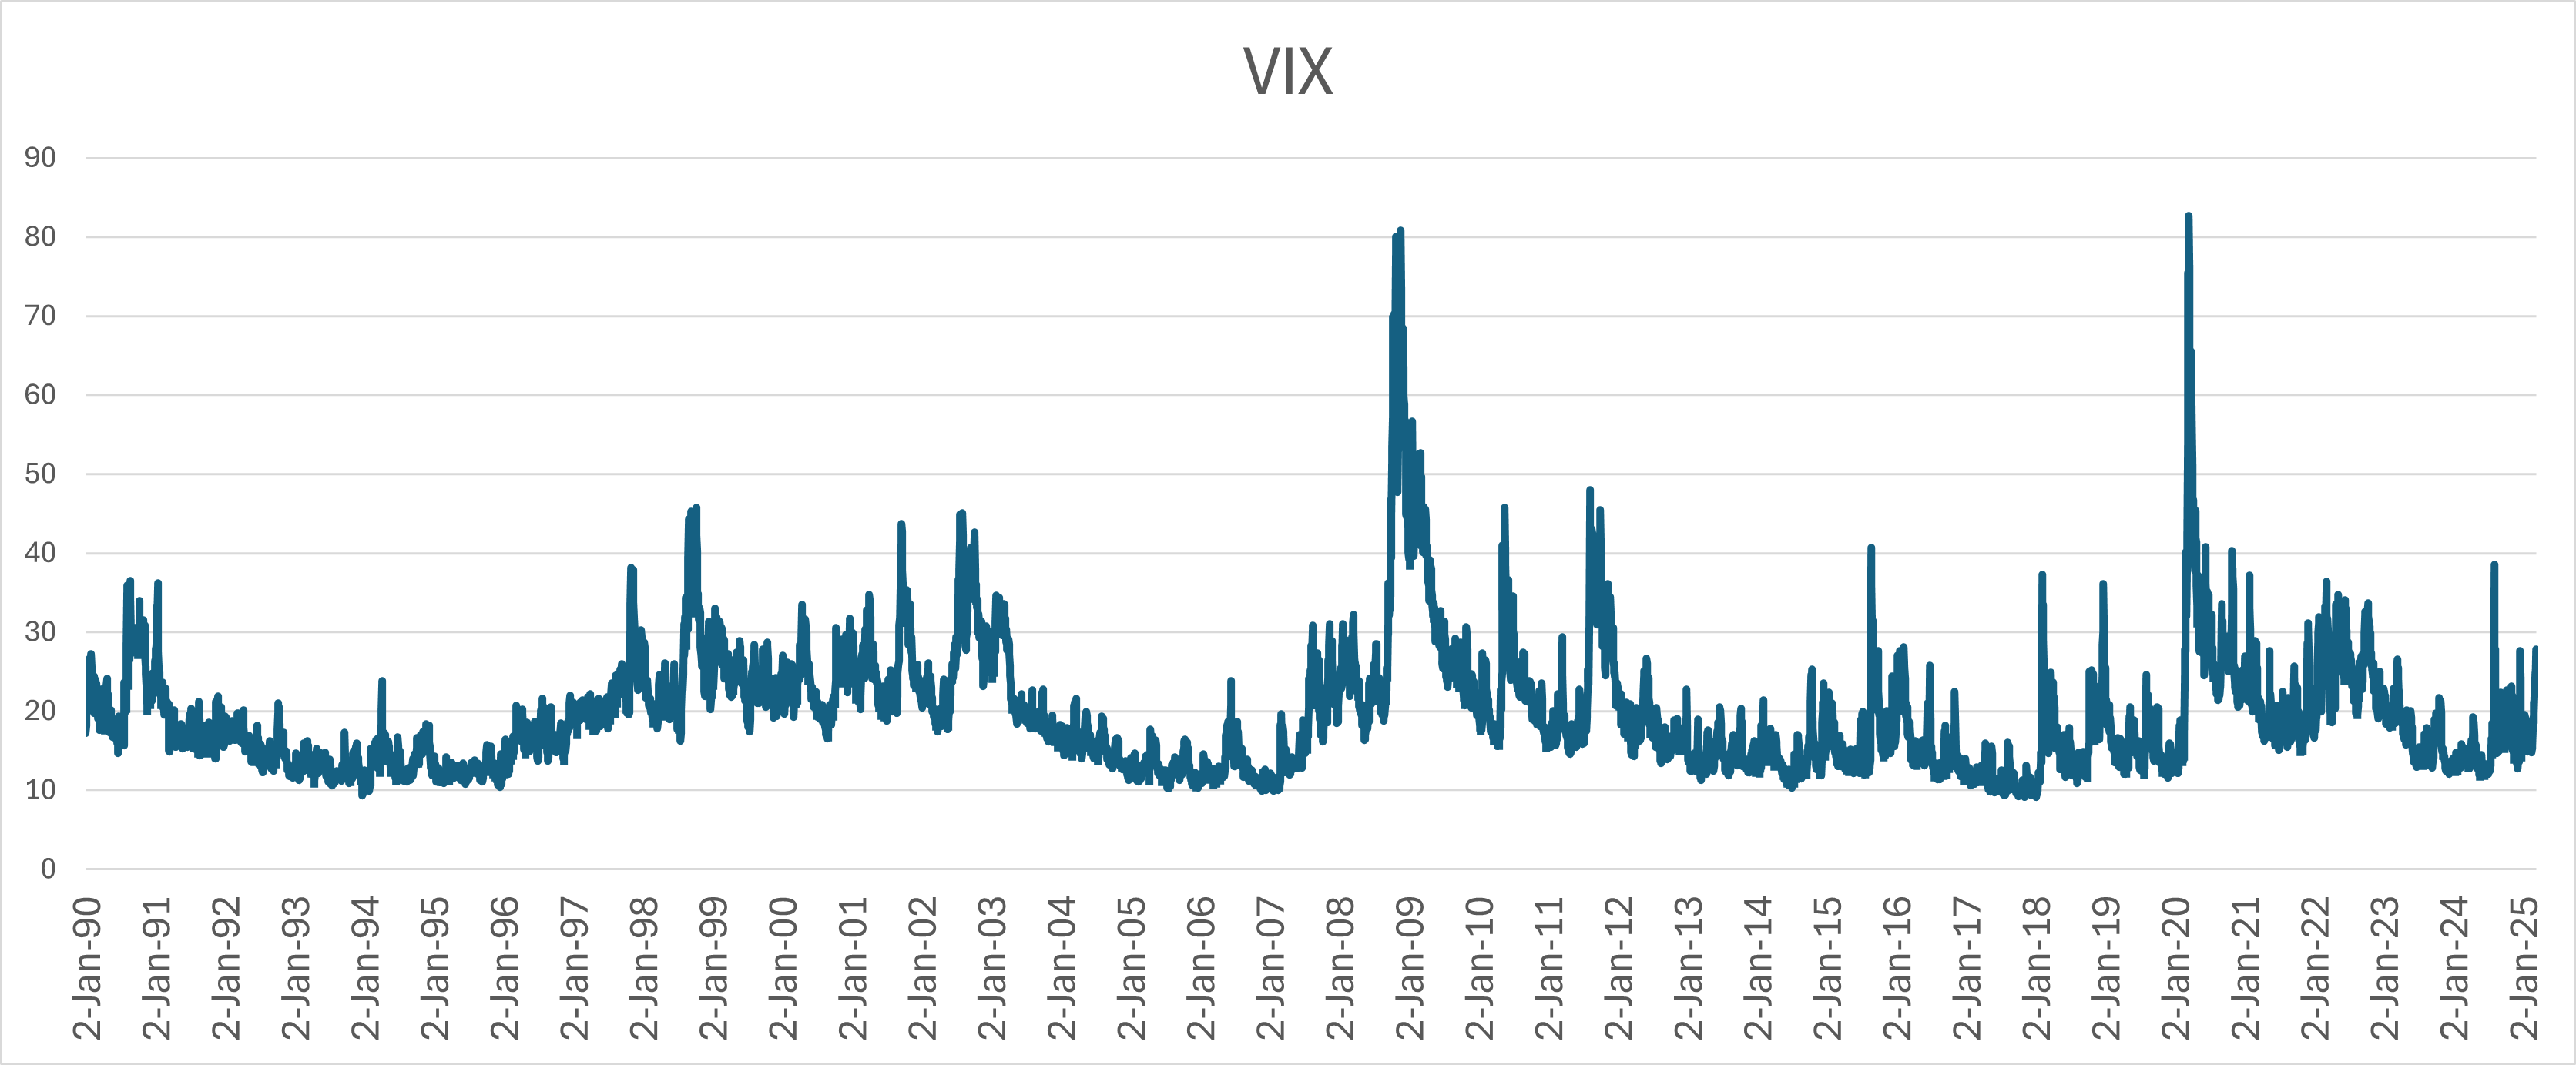
\includegraphics[width=\textwidth]{VIXOverTime.png}
\caption{VIX Historical Performance} \label{Fig-VIXHistorical}
\end{figure}
\noindent
There are a few interesting observations that can be made about the VIX alone:
\begin{itemize}
    \item It is highly volatile
    \item Appears to be range-bound
    \item Large spikes are transient
    \item Seems to revert to around 20
\end{itemize}
Next, let us view the VIX with the S\&P 500 index (SPX):
\\
\\
\begin{figure}[H]
\centering
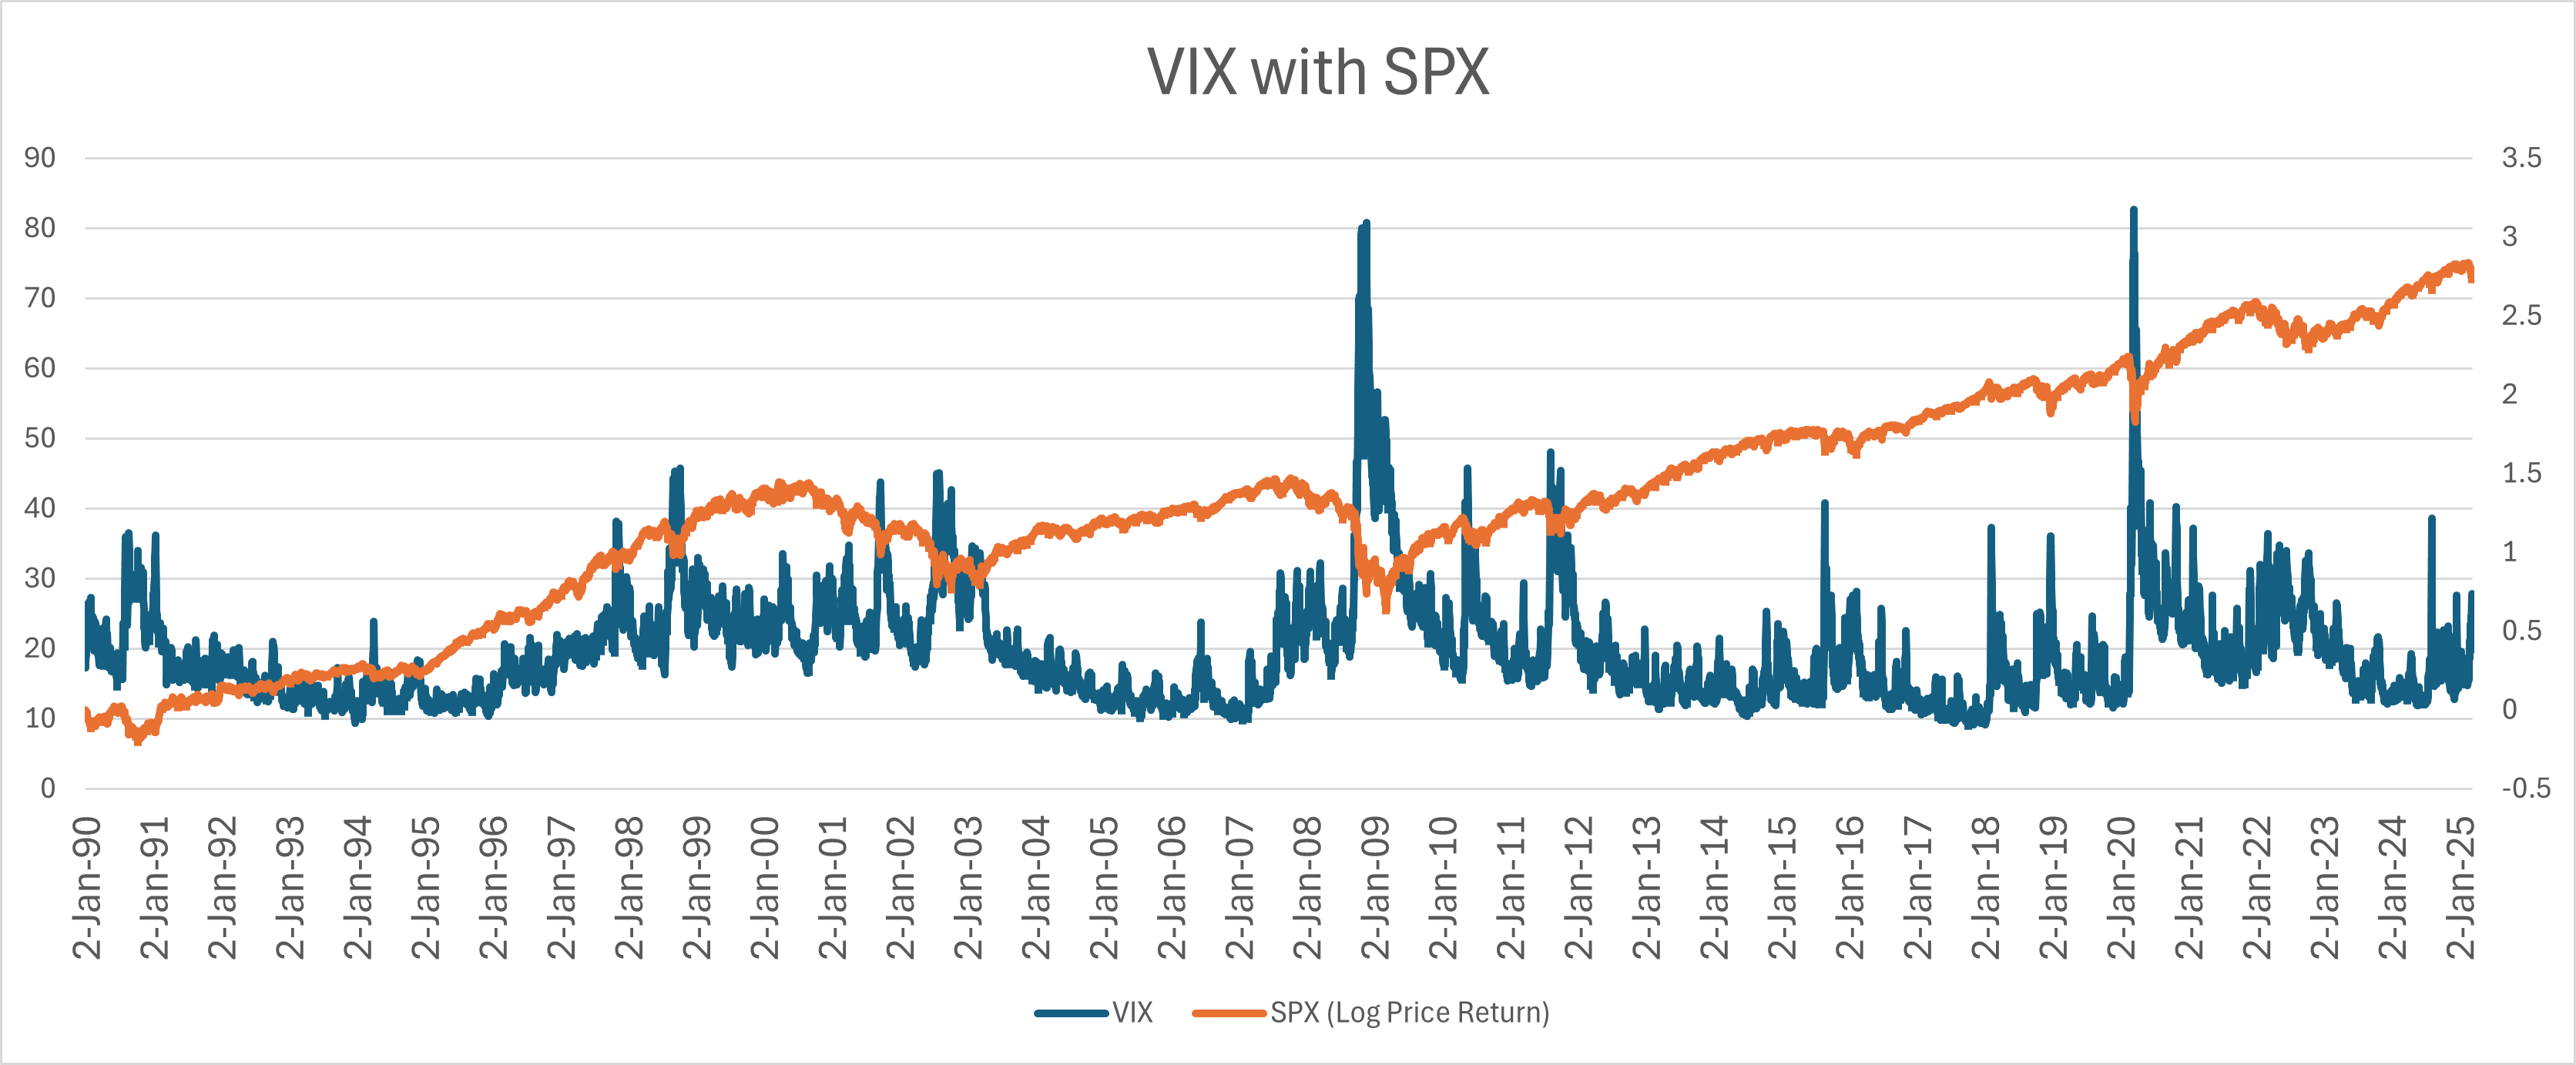
\includegraphics[width=\textwidth]{VIXandSPX.png}
\caption{VIX and SPX Historical Performance} \label{Fig-VIXSPXHistorical}
\end{figure}
\noindent
From this chart, it appears that the VIX increases in value when the SPX decreases in value. The VIX appears to be anti-correlated with the SPX. The following chart makes the anti-correlation with the SPX more apparent by removing the growth from the SPX.
\\
\\
\begin{figure}[H]
\centering
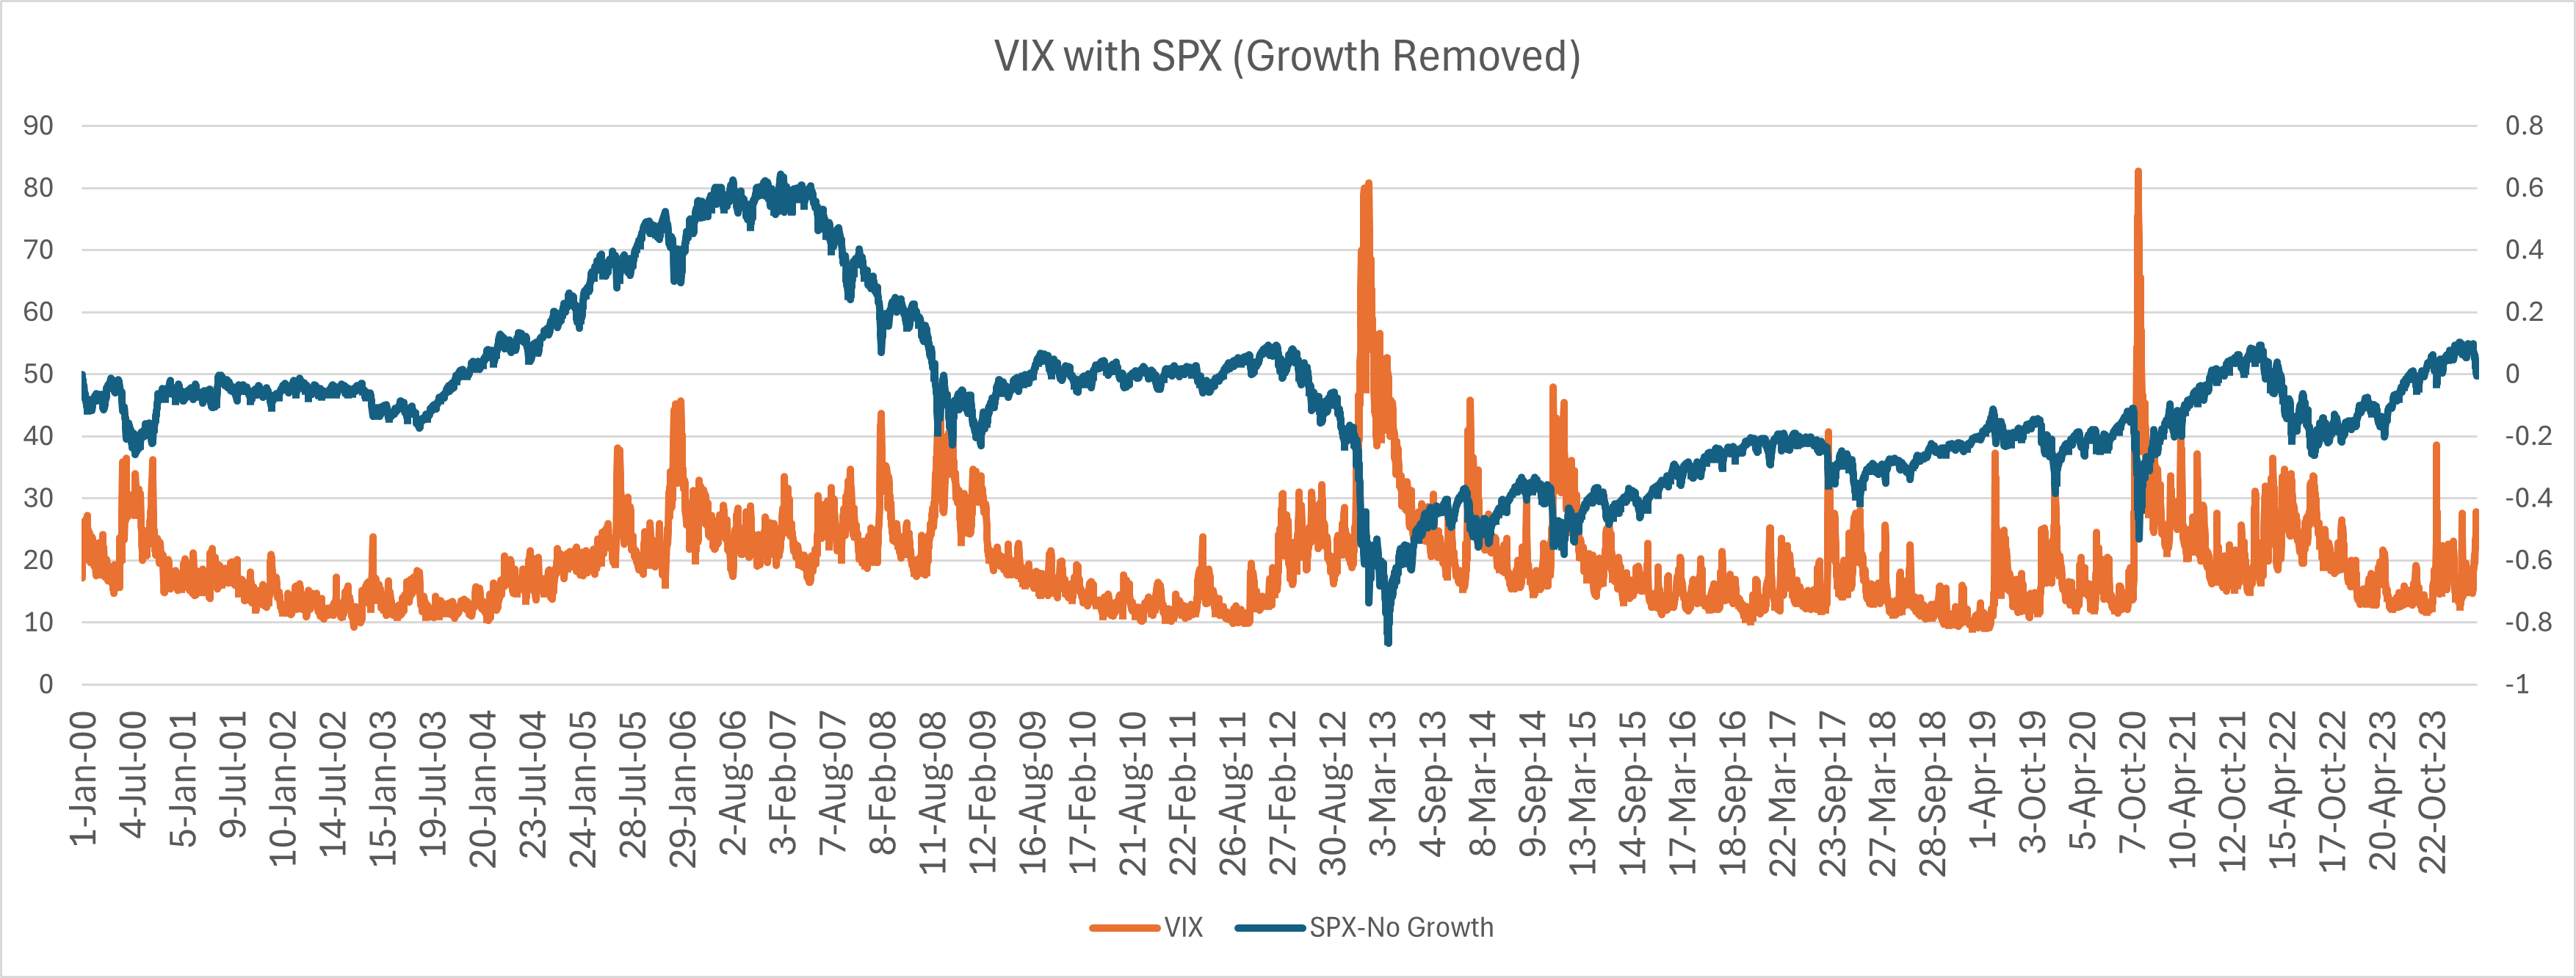
\includegraphics[width=\textwidth]{VIXandNoGrowthSPX.png}
\caption{VIX and SPX (Growth Removed) Historical Performance} \label{Fig-VIXAndSPXNoGrowth}
\end{figure}
\noindent
The above chart shows that the VIX is relatively low when SPX is relatively stable. The VIX increases sharply when the SPX experiences volatility. This behaviour is especially notable when the SPX decreases quickly. Hence the name "fear" index. The next section will investigate the correlation between the VIX and SPX realized volatility.

\section{VIX Versus Realized Volatility} \label{SigOfVIX-VIXVsReal}
As described in Chapter \ref{CalcVix}, the VIX is the annualized, option-implied 30-day volatility of the S\&P 500 index. This section will investigate whether the behaviour of volatility in the market. This section aims to answer the questions:
\begin{itemize}
    \item Does previous volatility correlate with future volatility?
    \item Is the VIX is a good predictor of future volatility?
    \item Does the VIX correlate with past volatility?
    \item Does the VIX correlate with the SPX?
\end{itemize} 
The simplest way to determine if an indicator is a good predictor of future results is to calculate an R-squared value. First, we will consider the question: Does previous volatility correlate with future volatility? The following chart is a graph of the previous 30-day volatility as a function of the future 30-day volatility.
\\
\\
\begin{figure}[H]
\centering
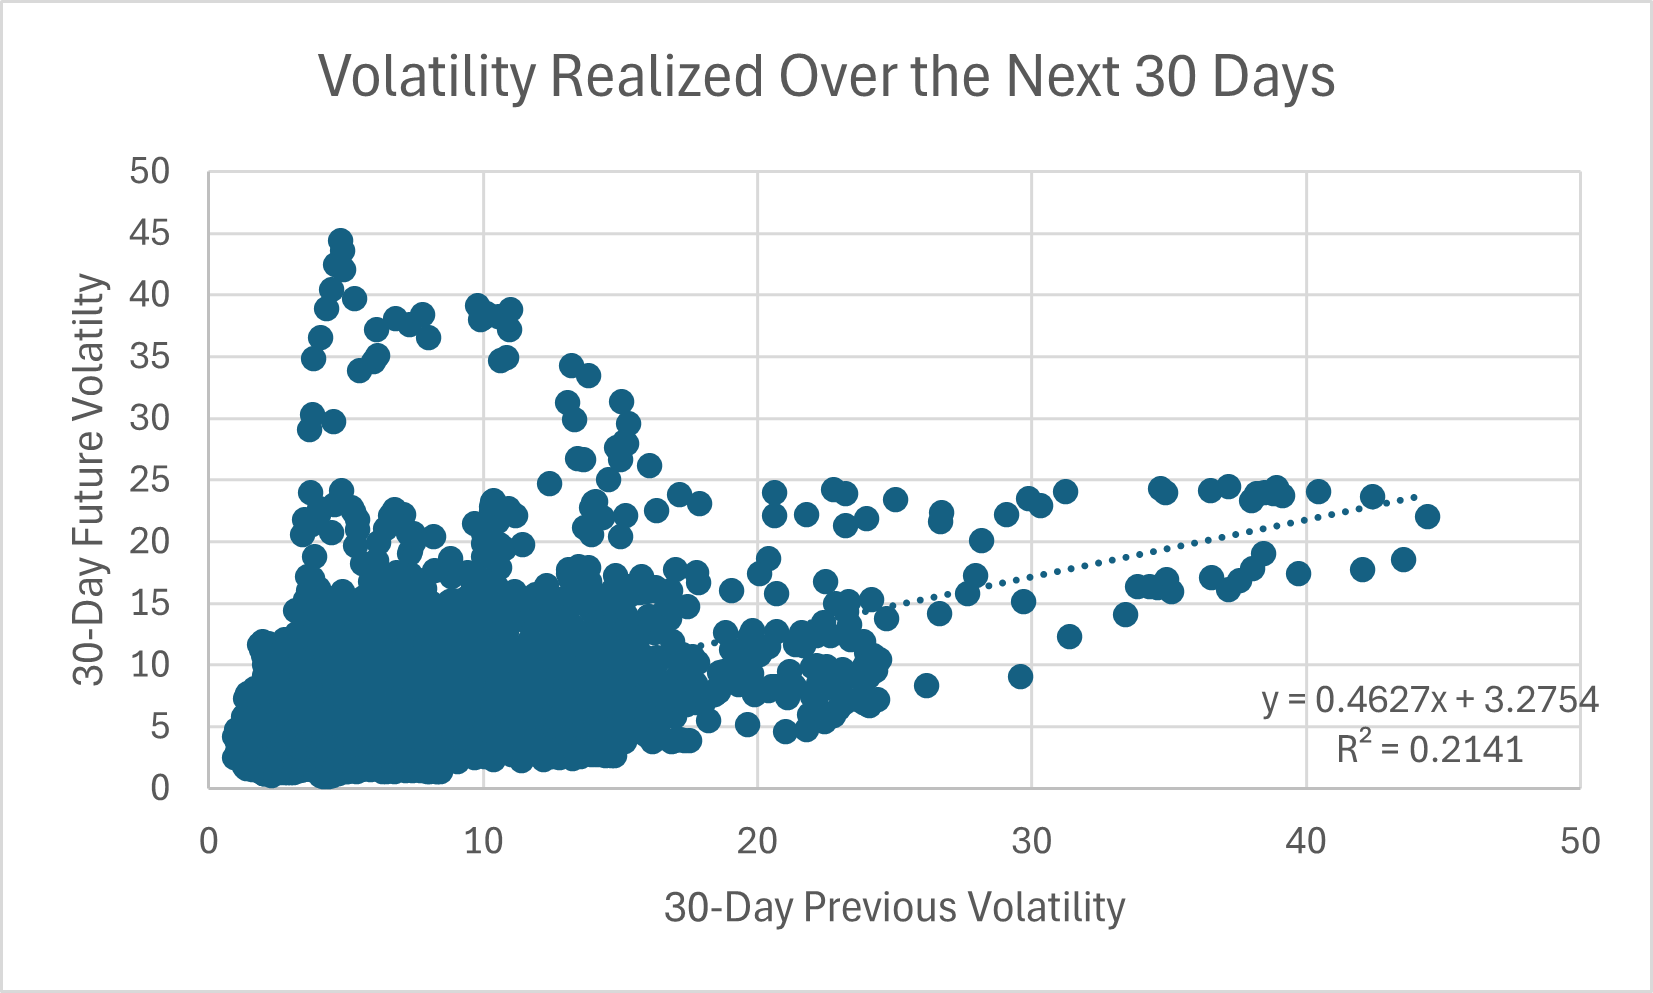
\includegraphics[width=\textwidth]{PreviousRealizedVolatilityVersusFutureRealizedVolatility.png}
\caption{Future Realized Volatility Versus Previous Realized Volatility} \label{Fig-FutureVersusPastVol}
\end{figure}
\noindent
This chart shows that there is some correlation between previous volatility and future volatility, but the correlation is not strong. Only 21\% of the future volatility can be explained by previous volatility. In other words, the previous realized volatility is a relatively poor indicator of the future realized volatility. Next, let's answer: Is the VIX a good predictor of future volatility? Since VIX is based on the prices of options that are determined by rational market participants, the VIX should correlate better with future realized volatility than previous realized volatility. The next chart confirms this theory.
\\
\\
\begin{figure}[H]
\centering
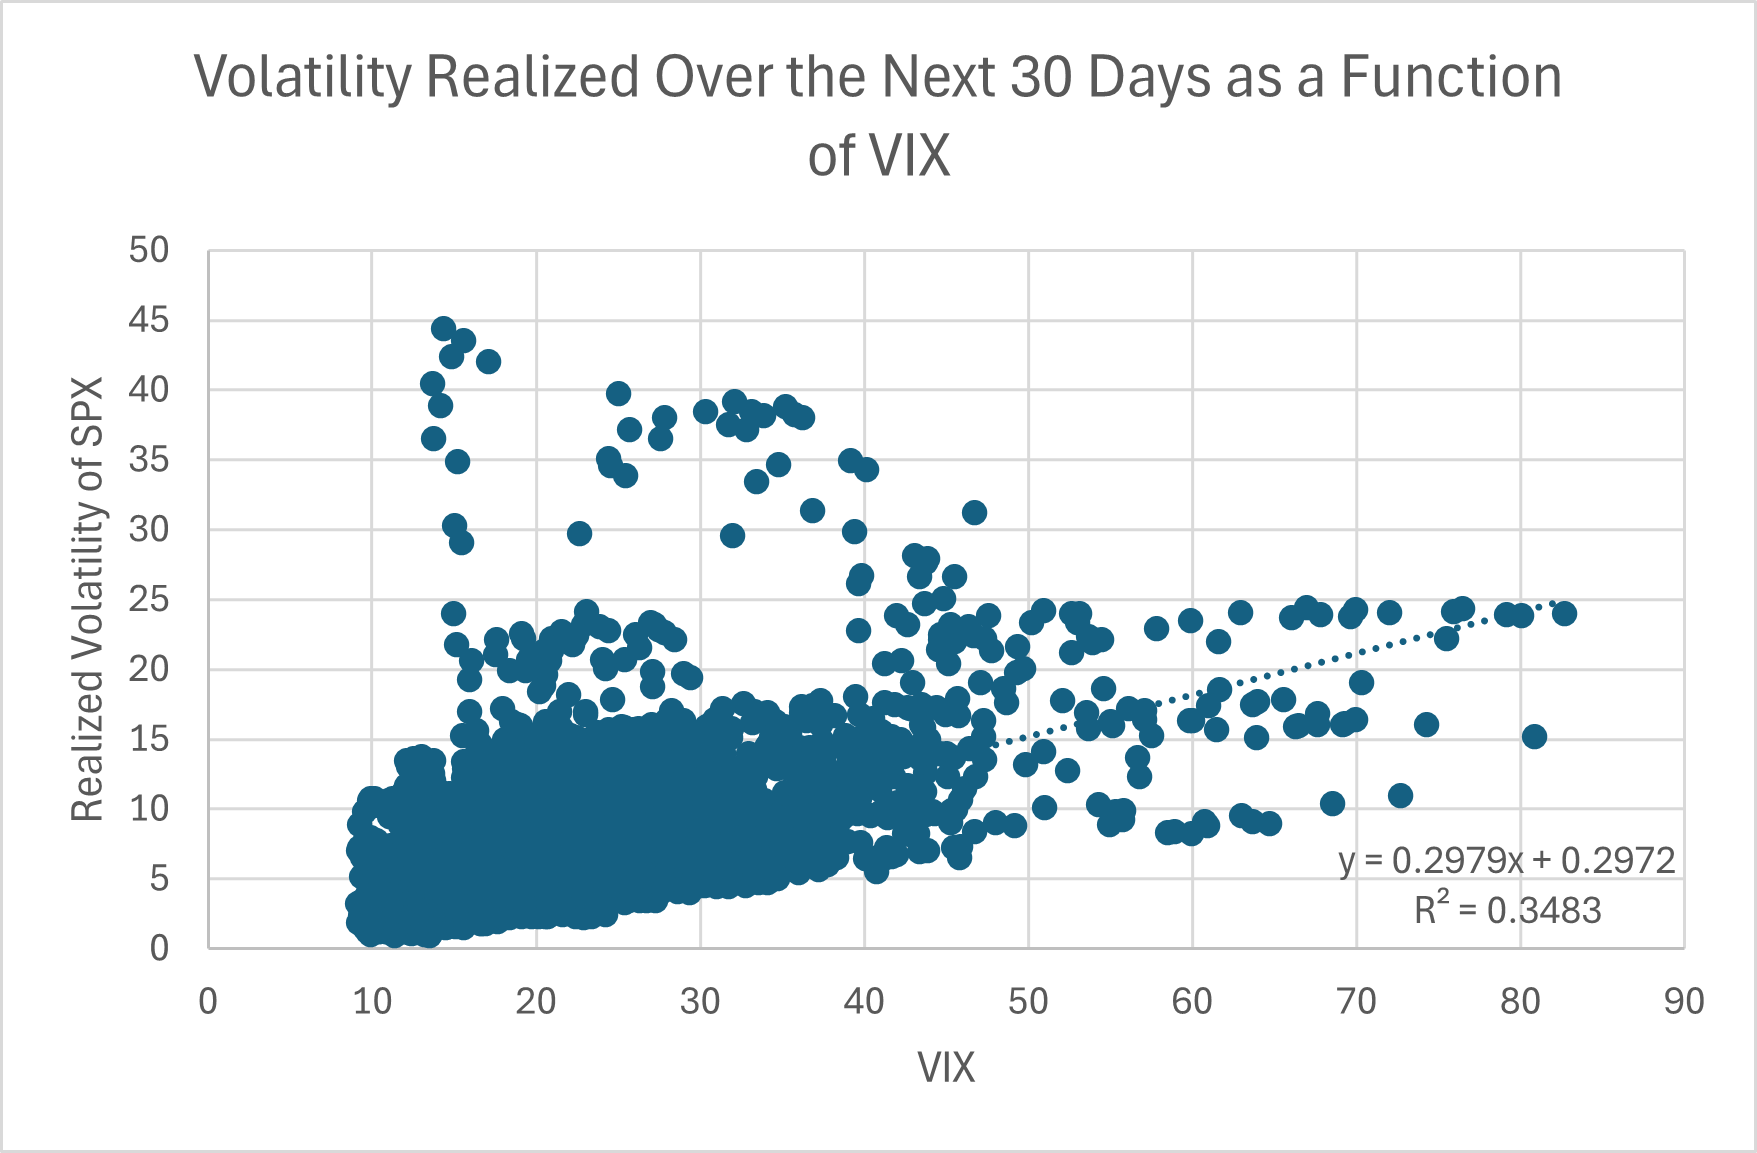
\includegraphics[width=\textwidth]{RealizedVolatilityVersusVIXForward.png}
\caption{Future Realized Volatility as a Function of VIX} \label{Fig-RealizedVolVersusVIX}
\end{figure}
\noindent
The R-squared value shows that 35\% of the realized volatility of the SPX can be explained by the VIX. While this correlation is significantly better than the correlation between previous realized volatility and future realized volatility, it is far from perfect. This implies that future realized volatility is difficult to predict.\\
\\
Lastly, let's see how much previous realized volatility impacts a market participant's expectations of future volatility (the VIX). The next chart graphs the VIX as a function of previous realized volatility.
\\
\\
\begin{figure}[H]
\centering
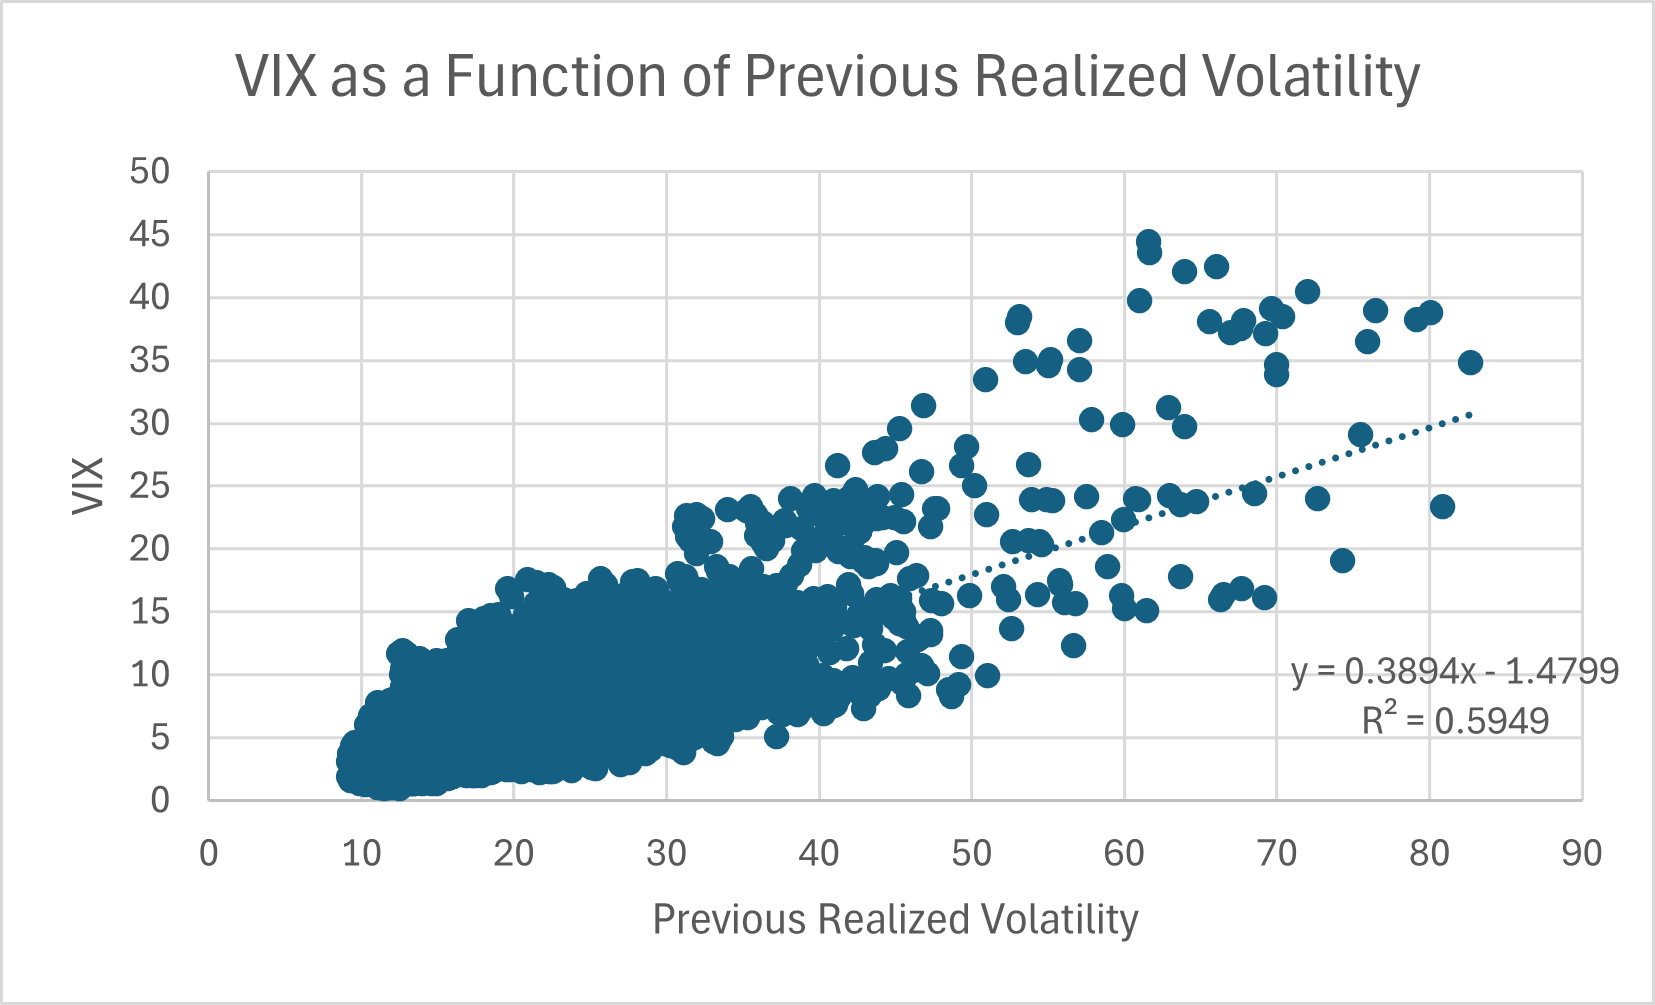
\includegraphics[width=\textwidth]{VIXVersusPreviousRealizedVolatility.png}
\caption{VIX as a Function of Previous Volatility} \label{Fig-VIXAgainstPrevVol}
\end{figure}
\noindent
Of the three scatter plots above, the VIX as a function of previous realized volatility has the highest correlation. The VIX predicts future volatility with a lower correlation than previous volatility predicts the VIX. In other words, the VIX functions more as a backwards-looking metric than as a forward-looking indicator. \\
\\
It is also useful to understand the correlation between the SPX and the VIX. The following chart shows the relationship between the daily move of the SPX and the daily move of the VIX.
\\
\\
\begin{figure}[H]
\centering
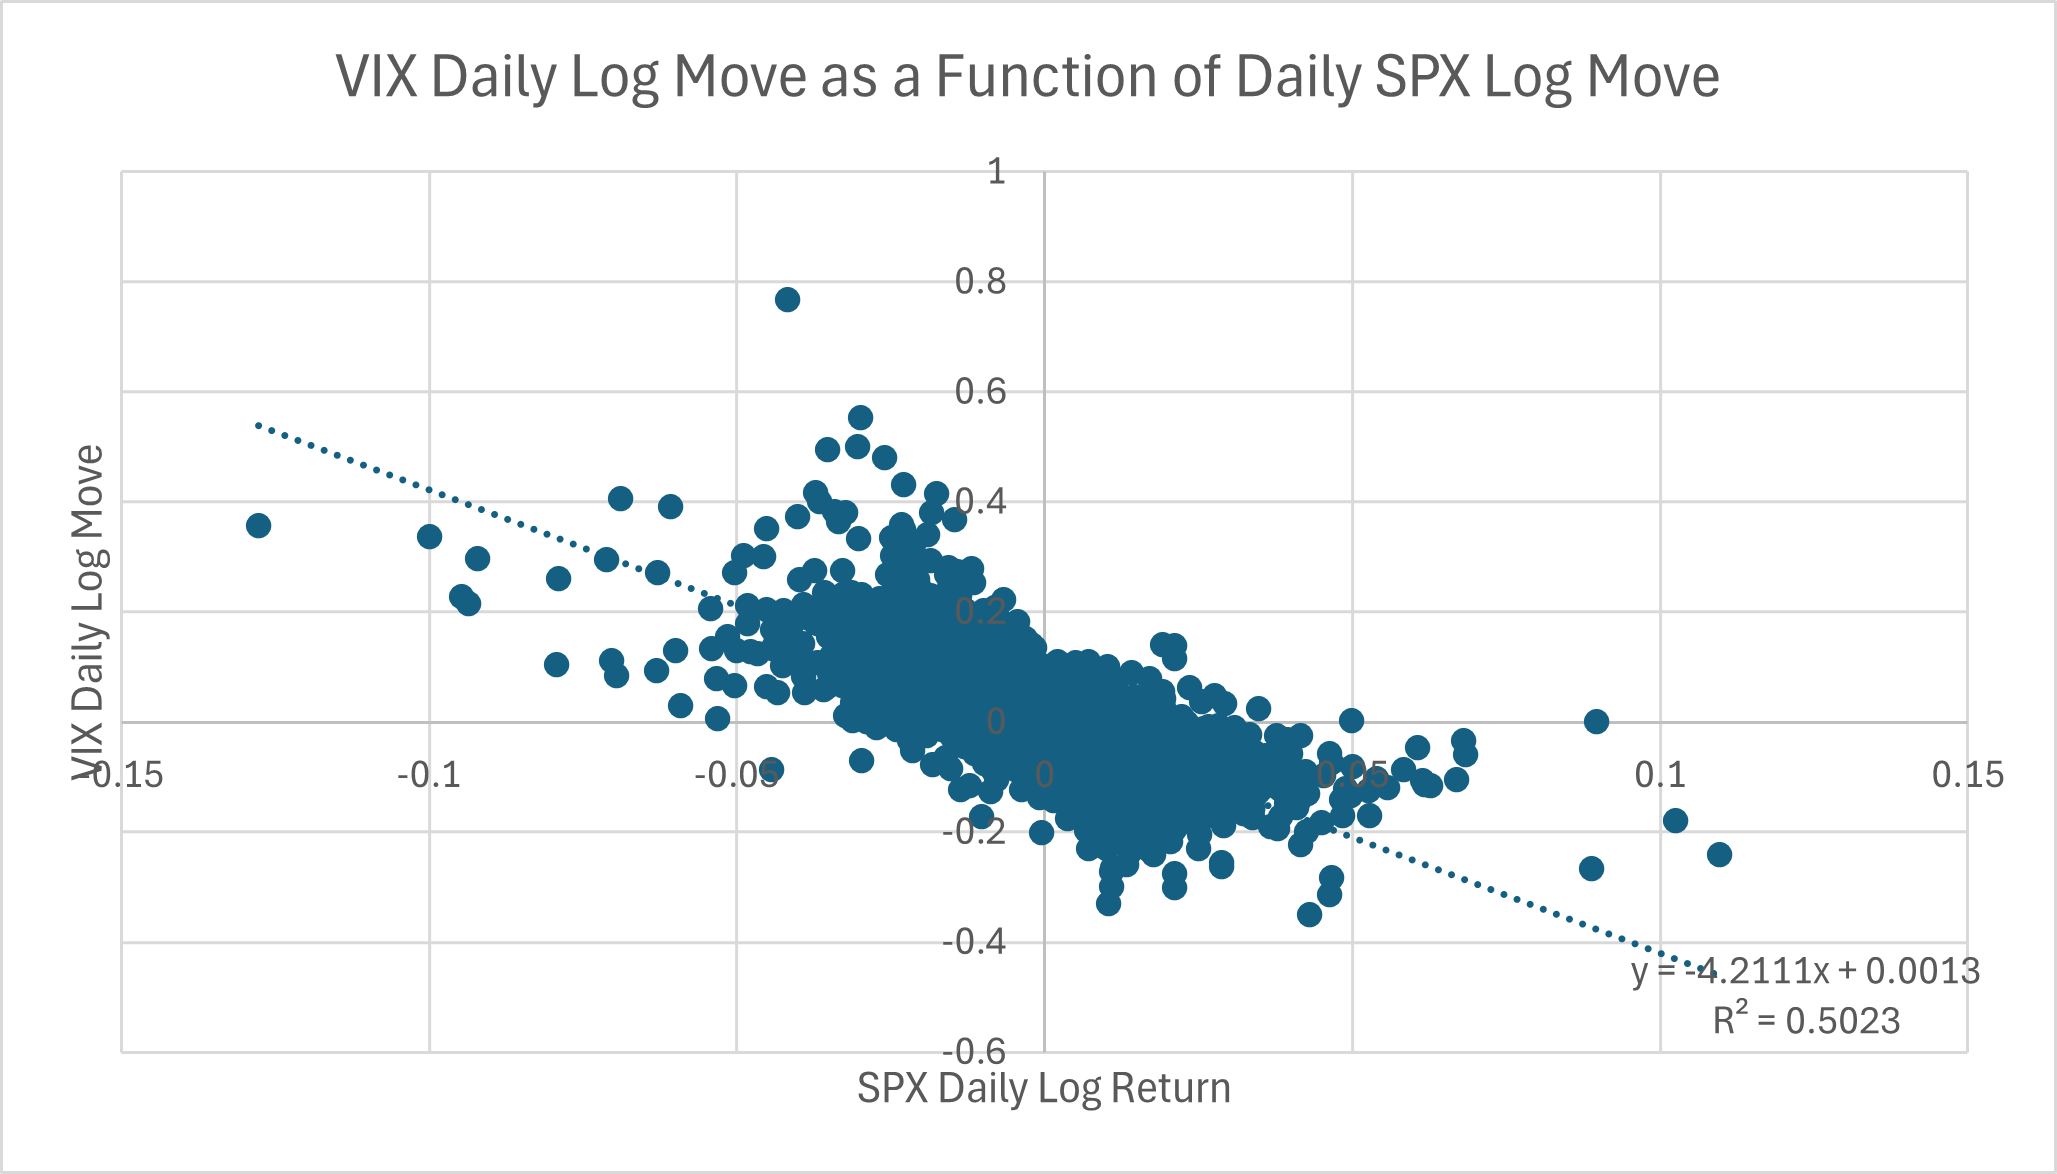
\includegraphics[width=\textwidth]{SPXCorrelationWithVIX.png}
\caption{VIXLogVersusSPXLog} \label{Fig-VIXLogSPXLog}
\end{figure}
\noindent
The chart above shows a clear negative correlation between the VIX and SPX. It is important to note that the strong negative correlation is not perfect. The SPX log move only explains 50\% of the VIX log move. The imperfect correlation will be important in a later section.\\

\section{VIX Behavior} \label{SigOfVIX-VIXBehave}
This section will discuss some of the different characteristics of the VIX. The VIX's behavior is prevalent throughout the pricing theory of VIX and its futures. This section will not attempt to explain the behavior, it will only review past data and observe different patterns and characteristics.\\

\subsection{Autocorrelation} \label{SigOfVIX-VIXBehave-AutoCorrel}
As described in section \ref{CalcVix}, the VIX is an instantaneous measure of the current market conditions. It is not dependent on its previous values. Despite this, volatility tends to cluster so even though the VIX doesn't directly depend on its previous value, it correlates well with its previous values. The following chart is the autocorrelation of the closing VIX each day.
\\
\\
\begin{figure}[H]
\centering
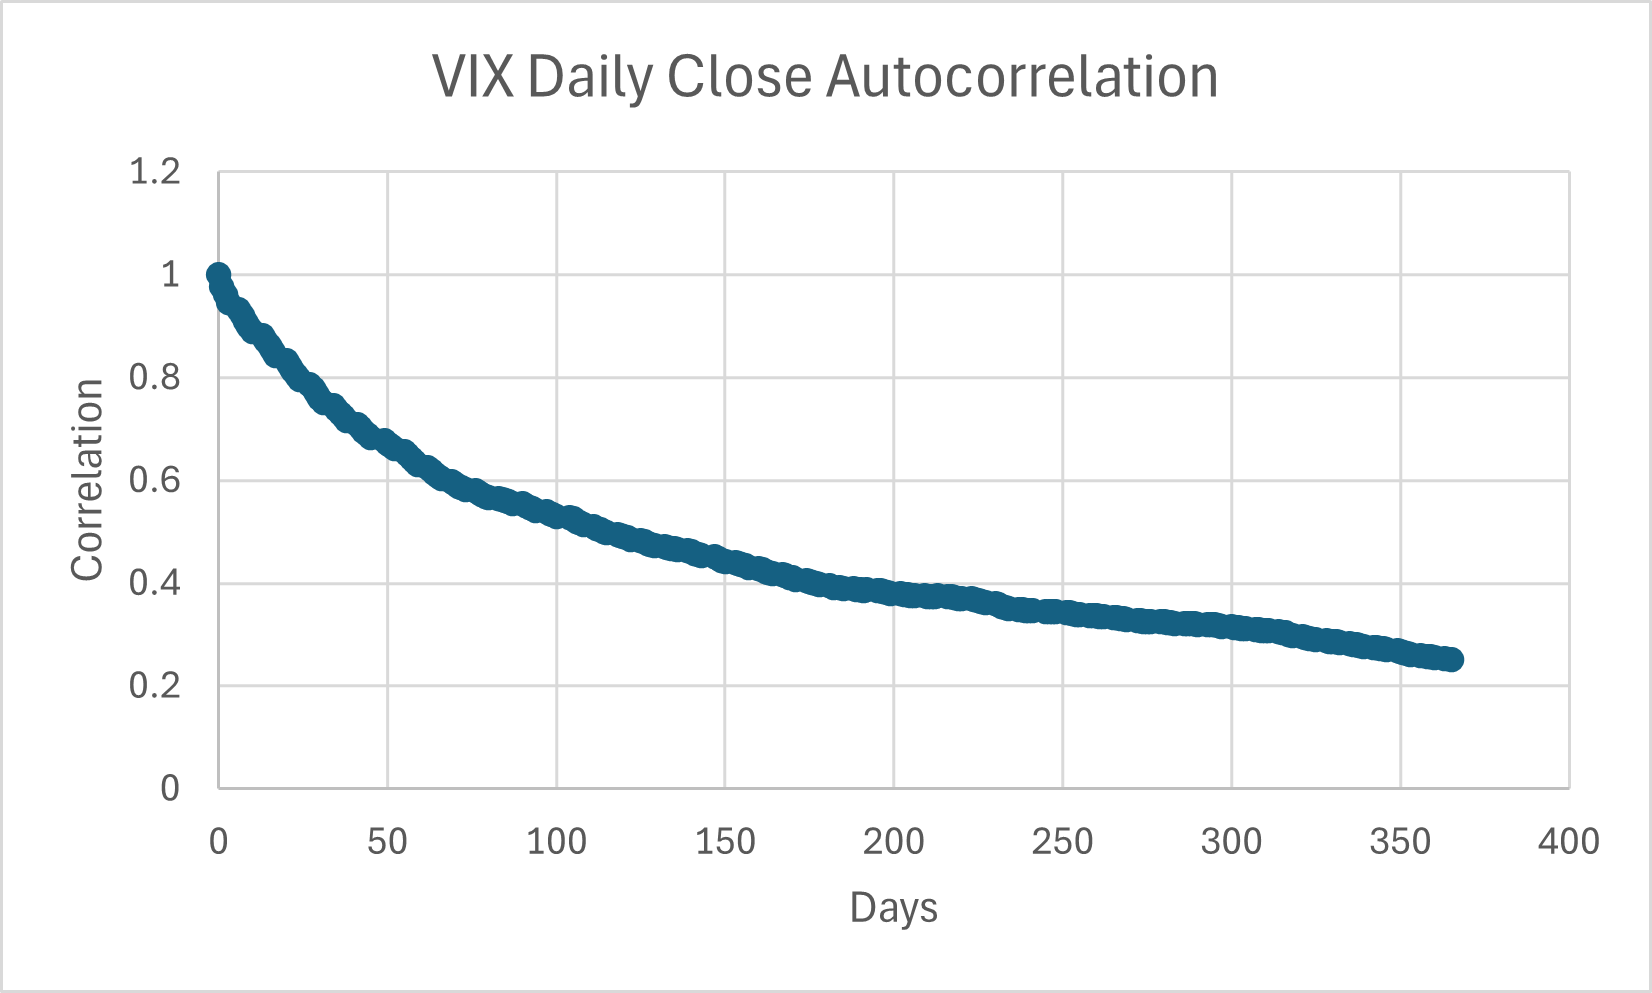
\includegraphics[width=\textwidth]{VIXAutocorrelation.png}
\caption{VIX Autocorrelation} \label{Fig-VIXAutocorrelation}
\end{figure}
\noindent
As shown, the VIX seems to have a short-term "memory" meaning that the VIX correlates strongly with prices in recent history, but not well with prices further back in history.

\subsection{Mean Reversion} \label{SigOfVIX-VIXBehave-MeanRev}
It can be observed from the VIX index values over time that when the VIX is relatively high, it tends to revert back to lower levels after a while. The opposite is true when the VIX is relatively low: when the VIX is low, it reverts back to a higher level. The following chart shows a plot of the daily return of the VIX as a function of the previous day's VIX level.
\\
\\
\begin{figure}[H]
\centering
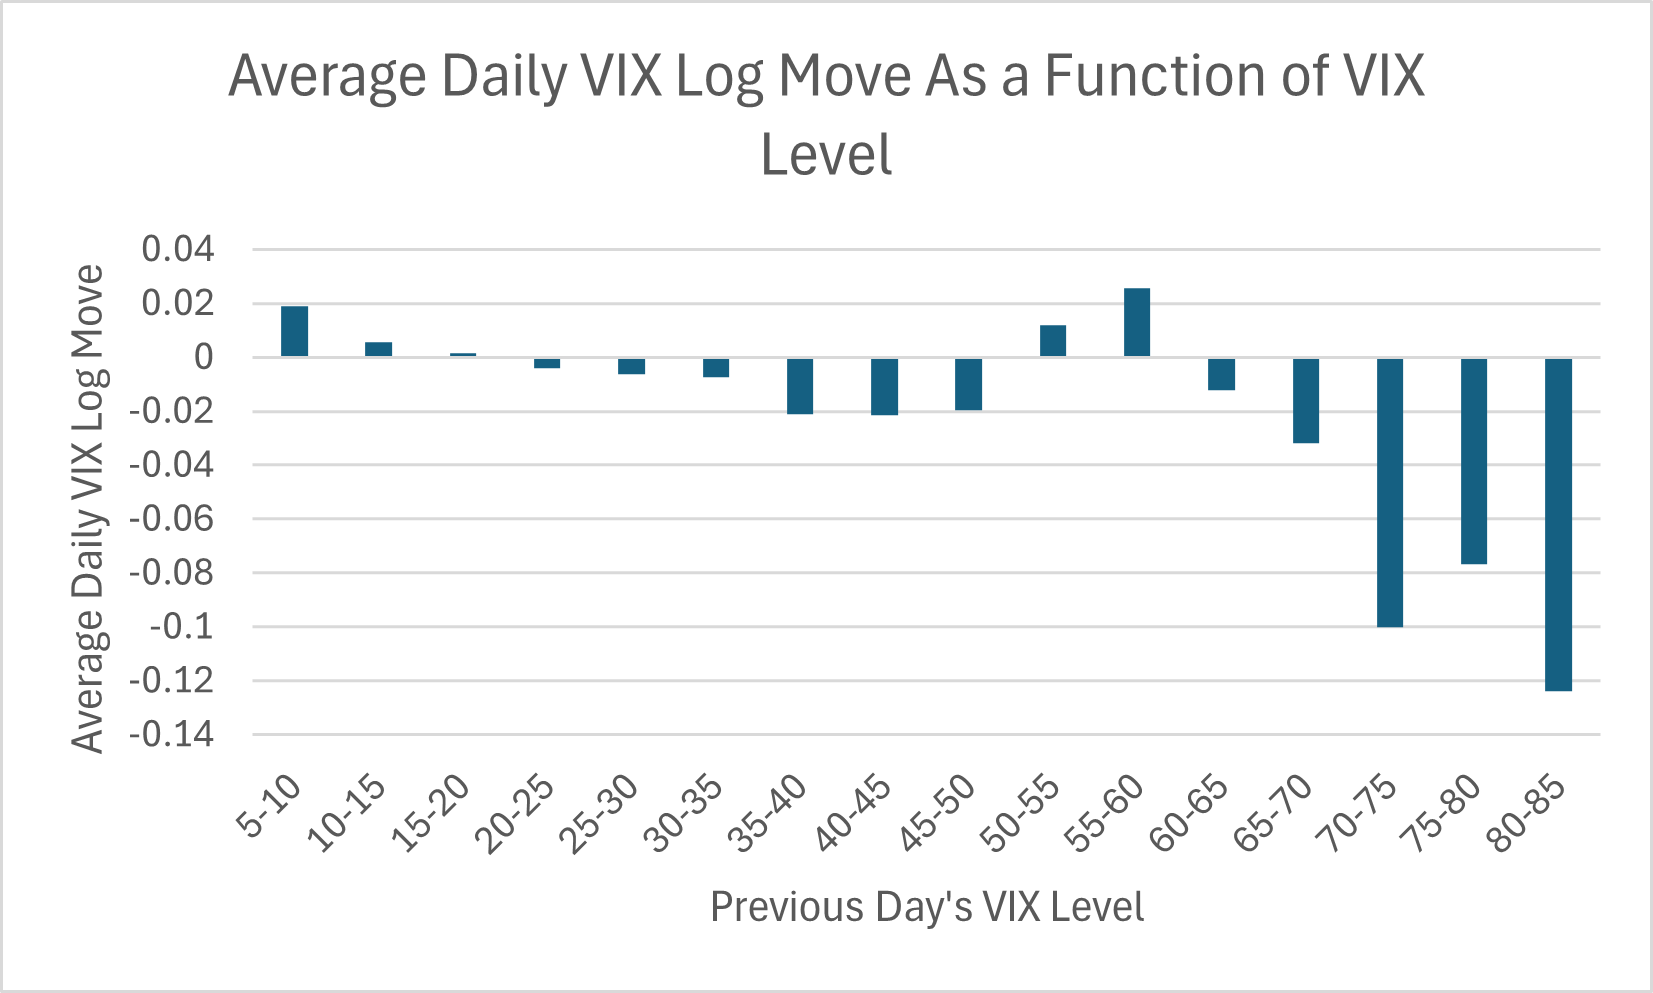
\includegraphics[width=\textwidth]{VIXDailyLogMoveAsAFunctionOfVIX.png}
\caption{VIX Log Move as a Function of VIX Level} \label{Fig-VIXLogFunctionOfVIX}
\end{figure}
\noindent
The chart shows that when the VIX is between 5-15, it tends to increase on average. When the VIX is between 15-20 (average), the VIX doesn't move much on average. When the VIX is above 20, the VIX tends to decrease on average. Note: The buckets where VIX are greater than 50 have a very low number of samples; this causes instability in the averages and explains why the buckets 50-50 and 55-60 have a positive value. \\
\\
Another way to view the mean reversion is by looking at the VIX as a function of the VIX in the past. The following chart is a plot of the VIX as a function of the VIX 30 days prior.
\\
\\
\begin{figure}[H]
\centering
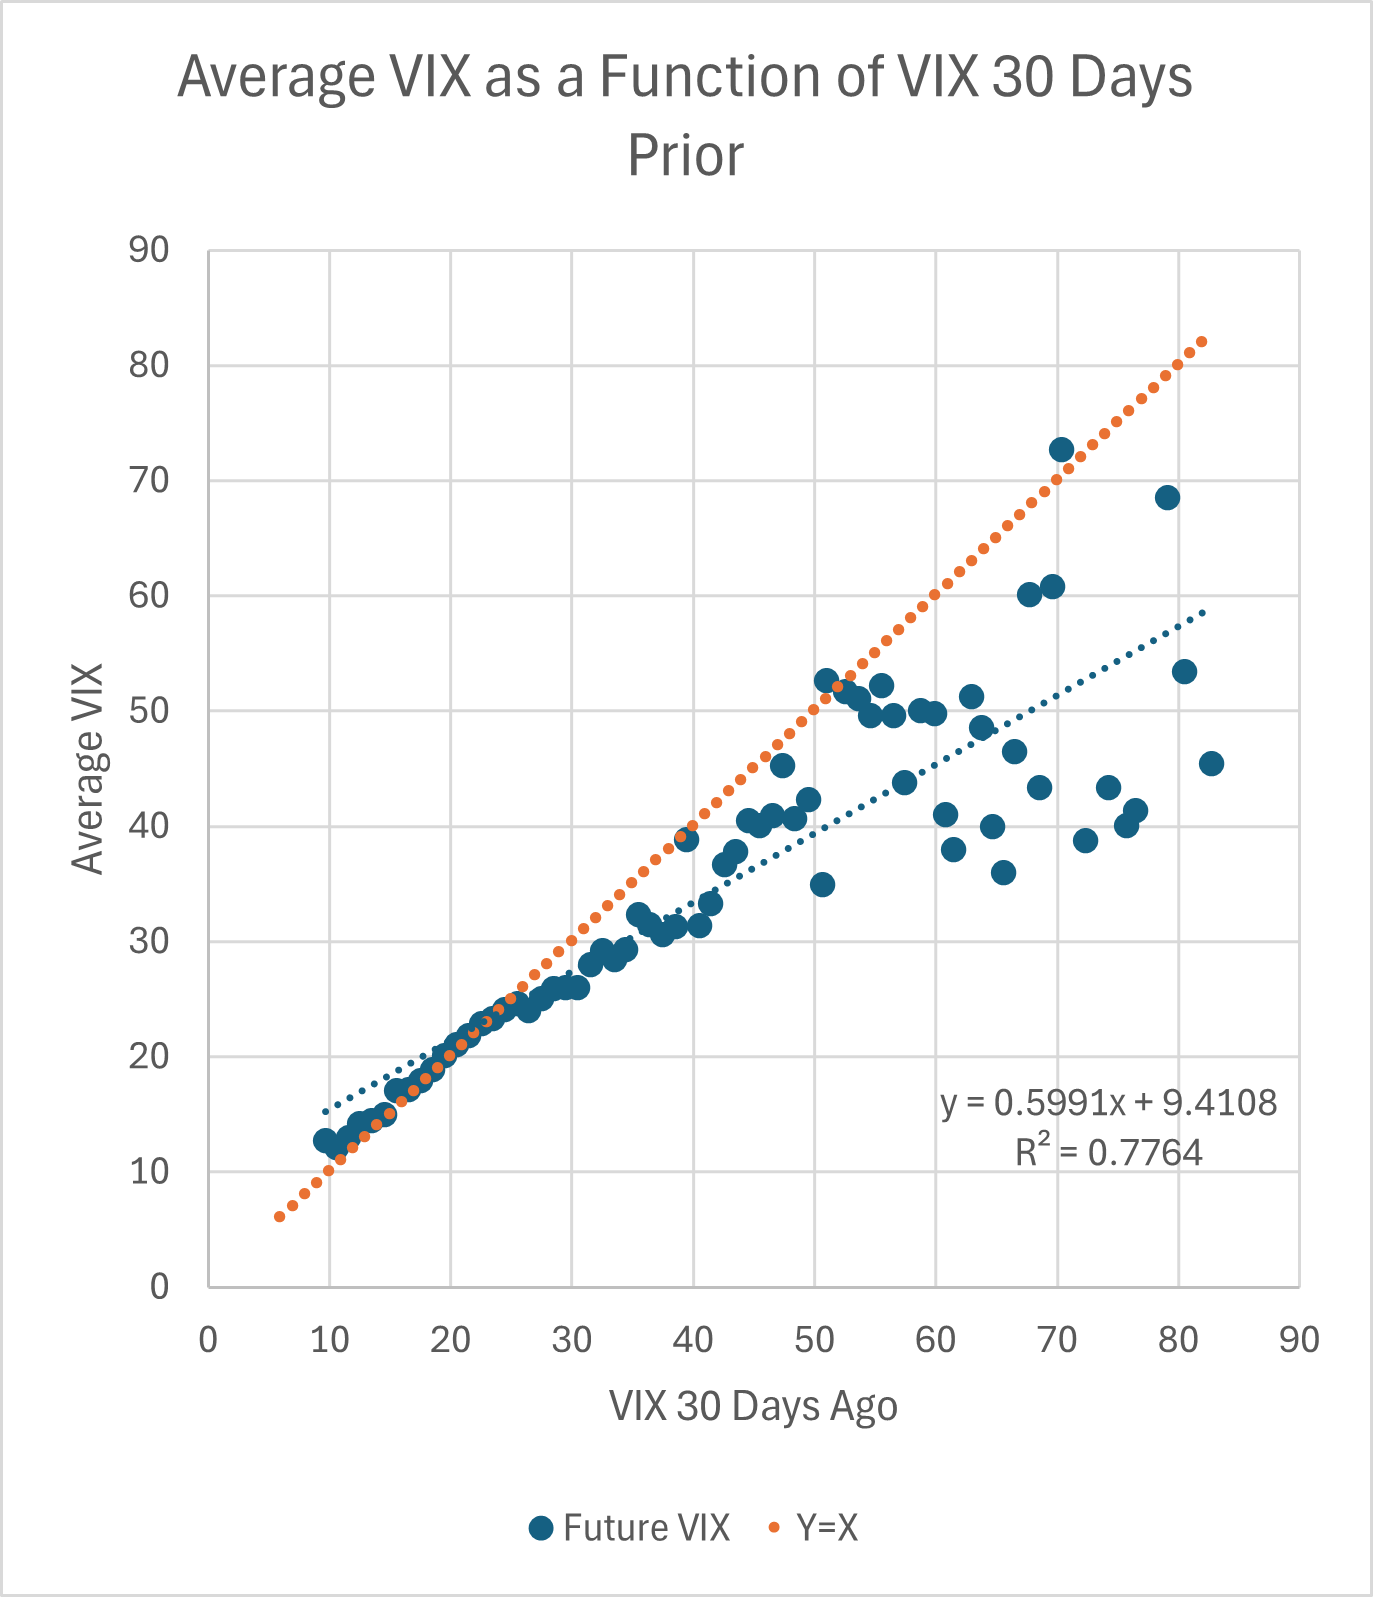
\includegraphics[width=\textwidth]{VIXAsAFunctionOfPriorVIX.png}
\caption{VIX as a Function of Prior VIX} \label{Fig-VIXFunctionOfPrevVIX}
\end{figure}
\noindent
Once again, the chart above shows that when the VIX is below 20 (the average, it tends to increase and when the VIX is above 20, the VIX tends to decrease.\\
\\
The same disclaimer applies: there are very few samples where the VIX is greater than 50. Therefore, the averages are somewhat unstable in those areas on the chart.


\section{Conclusion} \label{SigOfVIX-Conclude}
In conclusion the VIX:
\begin{itemize}
    \item Has low predictive power.
    \item Acts as a backward-looking metric of realized volatility.
    \item Is negatively correlated with the SPX.
    \item Is highly volatile.
    \item Is range-bound.
    \item Has transient spikes. 
    \item Mean-reverts.
\end{itemize} 


\chapter{Futures} \label{Futures}
\section{Introduction} \label{Futures-Intro}
Futures are a contract to purchase an asset at a later date at a pre-specified price. The futures discussed in this primer are cash-settled futures. For this reason, physically settled futures are not the focus of this section but they are used to provide some intuition behind the pricing of futures. This section will begin by describing S\&P 500 futures to provide some intuition of futures pricing. Next, this section will cover VIX futures and how they are priced. Lastly, this section will attempt to quantify the volatility risk premium. A reader comfortable with futures can skip to section \ref{Futures-VIXFuts}.
\\
\section{S\&P 500 Futures (/ES)} \label{Futures-ESFutures}
As stated in the introduction, futures allow two participants to agree to purchase an asset at a later date. There are four important factors to consider when trading futures:
\begin{itemize}
    \item The expiration date
    \item The futures price
    \item The spot price
    \item The cost of carry
\end{itemize}

\section{Expiration Date} \label{Futures-Expiration}
Exchange-traded futures (such as S\&P 500 futures (/ES) and VIX Futures (/VX)) have expiration dates predefined expiration dates.

\section{Futures Price} \label{Futures-FutPrice}
The futures price is the price that the future is currently trading at. When a transaction is made, the buyer is agreeing to buy the underlying on the expiration date at the current futures price.

\section{Spot Price} \label{Futures-Spot}
The spot price is the current price of the underlying. The spot represents the cost to purchase the underlying asset immediately.

\section{Cost of carry} \label{Futures-Carry}
The cost of carry is the cost of maintaining a position in the underlying obtained today until the expiration date. 

\section{Example} \label{Futures-Example}
The following example uses all of the terms above to build intuition about futures pricing:\\
If the \textbf{futures price} of an oil future is less than the cost of purchasing oil today (\textbf{spot price}) and paying for storage costs (\textbf{cost of carry}) until \textbf{expiration}, there exists an arbitrage opportunity for a market participant to short an oil future and purchase oil today.

\section{Applications of Futures to SPX and VIX} \label{Futures-Applications}
As stated in the introduction (section \ref{Futures-Intro}), SPX and VIX futures are cash-settled. This means that the futures settle to an index and the difference between the future price and the final settlement price (the price of the underlying upon expiration), is transacted between the buyer and seller of the futures.\\
\\
\subsection{SPX Futures} \label{Futures-Applications-SPX}
SPX futures settle to the S\&P 500 index. Purchasing an /ES future will provide exposure to the SPX index. After purchasing an SPX future, the buyer will profit if by expiration the SPX ends higher than the future price. If by expiration the SPX ends lower than the SPX future price, then the seller will profit.

\subsection{Arbitrage Conditions of SPX Futures} \label{Futures-Applications-Arb}
Since the S\&P 500 consists of roughly 500 companies weighted based on their market capitalizations, it is straightforward to gain exposure to the index by purchasing ETFs that track its performance. At first glance, it may appear that /ES futures can be arbitraged if the price of /ES deviates from the value of the SPX index by purchasing an S\&P 500 ETF and selling an /ES future to cancel the exposure. In this case, an arbitrageur would receive the dividends from the ETF (which reduce the SPX index value) and they would receive the difference between the futures price of /ES and the spot price of the ETF. \\
\\
However, purchasing ETFs requires capital upfront. Buying and selling futures does not require an initial capital outlay (other than margin requirements). This distinction means that the time value of money must be priced into the futures to prevent arbitrage. Otherwise, an investor could purchase SPX futures and use cash to purchase risk-free assets to create a risk-free return better than the market's. Therefore, SPX futures must be priced to include a risk-free yield on the cost of the S\&P 500 index. Including the risk-free rate in SPX futures pricing does not remove all of the arbitrage. \\
\\
Additionally, an investor must realize that futures traders are not entitled to dividends from the S\&P 500. Dividends reduce the value of the S\&P 500 index but do not compensate the holder of a futures position. Therefore, there may be an opportunity to purchase an S\&P 500 index and sell an /ES future to capture dividends. To maintain an arbitrage-free market, /ES futures must price in both the dividends and the risk-free rate. The relationship between these factors is captured in the following equation:
\begin{equation}
F = S \times e^{(r-y)T}
\end{equation} \label{Eq-CostOfCarry}
F is the futures price, S is the spot, e is Euler's constant, r is the risk-free rate, y is the projected dividend rate, and T is the time to expiration.\\
\\
This section provided some intuition assuming pricing is based on an arbitrage-free market. The next section will apply these ideas to VIX futures.

\section{VIX Futures} \label{Futures-VIXFuts}
VIX futures are different from most other futures because the underlying asset is not tradable. The only direct method to obtain exposure to the VIX is via futures or options. Therefore, it is difficult to price VIX futures based on the underlying using assumptions such as the arbitrage-free market assumption. Additionally, as shown in section \ref{SigOfVIX}, it is extremely difficult to predict the value of the VIX in the future based on data in the past. These two factors make it difficult to price VIX futures. This section will explain the basics of VIX futures pricing with the assumption that a fair value of the future VIX value is known. A complete description of how the fair value of the future VIX value can be obtained is out of the scope of this primer and is not described here. However, some intuition of VIX futures pricing is touched on in section \ref{Futures-Sensitivity}.

\subsection{The Fair Value of a VIX Future} \label{Futures-VIXFuts-Fair}
The fair value of VIX future is the value where the expected return of buying or selling the VIX future is 0. In other words, over a long time period, purchasing or selling VIX futures at the fair value would net 0 profit or loss. Assuming perfect knowledge of the probability distribution representing the future value of the VIX index at a time in the future, the fair value of a VIX future is the expected value of the probability distribution or the probability-weighted average of the probability distribution. This implies that the mean-reversion and range-bounded nature is priced into the fair value of a VIX future.
\\
\\
The following subsections explain why VIX futures typically trade at a premium rather than directly reflecting the expected future VIX value. We will take the perspective of a market participant hedging risk and a futures trader selling VIX futures.

\subsection{Hedging Market Risk Using VIX Futures} \label{Futures-VIXFuts-Hedging}
As shown in section \ref{SigOfVIX}, the VIX tends to increase sharply in value in response to a market downturn or market turmoil. This makes VIX futures a useful tool for hedging market risk and volatility risk. If hedging had no cost, an investor could obtain greater-than-market risk-adjusted returns by longing the market and hedging using VIX futures to hedge away risk. Since risk cannot be eliminated without cost, hedging with VIX futures must come with an expected cost over time. Under the assumption that it is not possible to obtain greater-than-market risk-adjusted returns, the expected returns from using VIX futures as a hedge should be equal to the expected returns of the risk reduction they provide. Note that this relationship is based on theory and is dependent on the efficient market hypothesis.

\subsection{Futures Trader Selling VIX Futures} \label{Futures-VIXFuts-Selling}
Section \ref{SigOfVIX} showed that the underlying VIX is very volatile. Selling futures on the VIX must entail significant risk. Since volatility itself is volatile and unpredictable, sellers of VIX futures demand compensation for the risk of being short volatility. Sellers of volatility expect the shorting of VIX futures to compensate for the risk they assume. For this reason, the risk-adjusted returns should be similar to the underlying asset that volatility describes. In the case of VIX, the underlying asset is the SPX index. Therefore, in an efficient market, the expected risk-adjusted returns of shorting VIX futures should match the risk-adjusted returns of holding the S\&P 500 over time.

\subsection{Risk Premium} \label{Futures-VIXFuts-Premium}
The compensation described in the previous sections is commonly referred to as Risk Premium. The previous sections described the fair value of a VIX future and compensation for taking risk selling VIX options. These two ideas can be combined into a simple equation to price VIX futures:
\begin{equation}
F = E[VIX] + P
\end{equation} \label{Eq-VIXPricing}
$F$ is the futures trading price, $E[VIX]$ is the fair value of VIX futures or the expected value of the VIX, and $P$ is the risk premium of selling VIX futures.\\
\\
Note that this definition relies on the premise that the market is efficient and the expected VIX is correct on average. The long-term average of risk-premium can be estimated, but unless it can be precisely calculated, the expected VIX is unknowable based only on the futures price and the spot price.

\section{Quantifying Risk Premium} \label{Futures-Quantify}
Historical futures data can be analyzed to quantify the risk premium. While historical data may not be representative of future results, it may be valuable to review historical data as a basis to understand potential future risks. The fundamentals laid out previously in this section intends to explain why shorting volatility has a positive expected value. This section aims to provide a rough estimate of the expected value of shorting volatility futures. \\
\\
The following chart is a chart of the average VIX futures price as a function of the days to expiration. The details behind how the data was smoothed are provided in Appendix A. 
\\
\\
\begin{figure}[H]
\centering
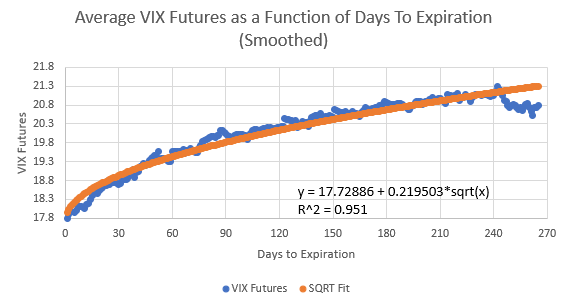
\includegraphics[width=\textwidth]{VIXFuturesAsAFunctionOfDaysToExpiration.png}
\caption{Average VIX Futures Price as a Function of Days to Expiration} \label{Fig-AvgVIXDaysToExpiration}
\end{figure}
\noindent
The chart above shows the decay pattern of the VIX futures. As shown, the a square root fits the graph very well. The idea of derivatives decaying in square root time may be familiar to option traders familiar with the Black-Scholes model. From the graph above, it is clear that the expected returns of shorting volatility increase as the time to expiration decreases. Notably, the sensitivity of the futures price to the spot VIX increases as the time to expiration decreases. In other words, as time to expiration decreases, the volatility of a short VIX position increases as well as the expected returns.\\
\\
From the equation on the chart above, it is possible to determine an average expected return from shorting VIX futures per day based on the days to expiration. As stated previously in this section, historical data may not be an accurate representation of future events. This data is being used to provide estimates of expected returns. The next section will use information from the historical results to create option strategies that exploit the VIX risk premium.

\section{Sensitivity of VIX Futures to the Spot VIX} \label{Futures-Sensitivity}
Since VIX futures settle to the spot VIX, there must be some relationship between the VIX futures and the spot VIX. As the time to expiration of a VIX futures contract approaches 0, the VIX futures price should approach the spot VIX. Similarly, as the time to expiration of a VIX futures contract approaches 0, the VIX futures price should change by an equal amount.\\
\\
Due to the autocorrelation of the VIX with itself shown in section \ref{SigOfVIX-VIXBehave-AutoCorrel}, a similar effect should hold for VIX futures with a non-zero, but short time to expiration.\\
\\
However, for longer times to expiration, the autocorrelation of the VIX with itself is very weak. In these cases, it makes sense to rely on other more complicated methods to predict expected volatility as well as the mean-reverting behavior of VIX described in section \ref{SigOfVIX-VIXBehave-MeanRev}. Therefore, a contract that has, for example, 8 months to expiration may not move much if the VIX goes from 20 to 80 because it is expected that the VIX will revert to its mean within the 8 months.

\section{Contango, Parity, and Backwardation} \label{Futures-ConBackPar}
Interestingly, unlike the /ES futures described above, the equation in section \ref{Futures-VIXFuts-Premium} does not include the spot VIX, only the expected VIX by expiration. This may be surprising because VIX futures ultimately settle to the spot VIX (or the special opening quotation of the VIX). This leads to interesting behavior in VIX futures that - using the ideas from the /ES futures - could only be explained with 0\% or negative interest rates. \\
\\
The following subsections will detail the names of the different relationships that futures can have with the spot as well as explain how SPX futures and VIX futures may differ during these conditions.

\subsection{Contango} \label{Futures-ConBackPar-Con}
Contango describes the relationship between the spot and the futures when the futures price is higher than the spot.\\
\\
The VIX futures are in contango a majority of the time. Using the equation from section \ref{Futures-VIXFuts-Premium}, the VIX is in contango whenever the expected VIX plus the risk premium is greater than the spot VIX. A majority of the time, the VIX is in contango because the expected VIX is generally close to or higher than the spot VIX.\\
\\
/ES futures are in contango when the risk-free rate is greater than the expected dividend yield of the S\&P 500. As described in section \ref{Futures-Applications-Arb}, this is because the risk-free rate and the dividend yield work against one another when pricing S\&P 500 futures.

\subsection{Parity} \label{Futures-ConBackPar-Par}
Parity describes the relationship between the spot and the futures when the futures price is the same as (or very close to) the spot price. \\
\\
VIX futures are in parity when the expected VIX lower than the spot VIX by nearly the risk premium demanded by the sellers of VIX futures.\\
\\
/ES futures are in parity when the risk-free rate and the expected dividend rate are nearly equivalent to one another.

\subsection{Backwardation} \label{Futures-ConBackPar-Back}
Backwardation describes the relationship between the spot and the futures when the futures price is lower than the spot.\\
\\
VIX futures are in backwardation when the expected VIX is less than the VIX spot by more than the risk premium demanded by VIX sellers. This tends to be the case after periods of high realized volatility. This is because a reversion to mean is expected soon after a period of realized volatility (sustained high volatility is not expected). Section \ref{SigOfVIX} touched on the idea that the VIX rarely spikes and when it does, it usually falls very quickly to lower levels.\\
\\
/ES futures are in backwardation when the expected dividend yield is higher than the risk-free rate. This generally occurs when interest rates are near zero or negative.

\section{Common Myth: Buy Backwardation, Sell Contango} \label{Futures-Myth}
Since the VIX futures eventually settle to the spot VIX, there is a common misconception that shorting VIX futures is profitable during periods of contango and buying VIX futures is profitable during periods of backwardation. This idea assumes that the spot VIX will not experience significant movement between the present day and the futures contract's expiration.\\
\\
This idea implies that market participants do not accurately price the tendency of the VIX to revert to its historical mean during periods of backwardation. In other words, the idea that buying VIX futures is profitable during backwardation implies the market is inefficient during periods of backwardation.\\
\\
Since the VIX futures are rarely in backwardation, there is not enough data to provide strong empirical evidence for/against the claim that longing VIX futures has positive expected returns. However the same argument in \ref{Futures-VIXFuts-Selling} still applies. Longing VIX futures during backwardation is a viable hedge to market drawdowns and continued volatility. An investor who goes long VIX futures during backwardation would profit if expected volatility remains higher than the market expects over the period of the futures contract. This means that a seller of VIX futures will continue to demand a risk premium even during periods of backwardation.

\chapter{VIX Options} \label{Options}
\section{Introduction} \label{Options-Intro}
This section will explain some concepts of options that are relevant to long-term investing in short volatility strategies. This section covers the surface of option pricing and is not intended to be comprehensive. Basic knowledge of options is required prior to reading this section.

\section{The Underlying} \label{Options-Underlying}
VIX options are cash-settled, European-style options meaning they are not physically delivered and they can only be exercised on the expiration date. Therefore, the options are priced as if the underlying is the VIX futures with the same expiration date as the options rather than the spot VIX. For this reason, the option-implied forward price of the VIX will always be nearly exactly the VIX futures price.

\section{Intrinsic and Extrinsic Value} \label{Options-IVEV}
The value of an option can be divided into two components: Intrinsic and Extrinsic value. 

\subsection{Intrinsic Value} \label{Options-IVEV-Intrinsic}
Intrinsic value is the value of an option if it were to be exercised immediately. For puts, the intrinsic value is the difference between the strike price and the VIX futures. Generally, options will always trade at or above their intrinsic value.

\subsection{Extrinsic Value} \label{Options-IVEV-Extrinsic}
Extrinsic value is the difference between the option price and the intrinsic value. When an option expires, all that is left is the intrinsic value. Therefore, if the underlying does not move until expiration, the extrinsic value decreases to zero. \\
\\
The methods for calculating extrinsic value vary and are out of the scope of this primer. As a slightly inaccurate and pessimistic heuristic, this primer will assume extrinsic value is a non-recurring cost of the exposure that options provide. The view that extrinsic value is a cost is slightly inaccurate because extrinsic value represents the value of the asymmetric payoff. Taking the view that extrinsic value is a cost of exposure is a pessimistic view because it doesn't consider the convexity of the payoff for the holder of an option.

\section{Put-Call Parity} \label{Options-PutCall}
\subsection{Description} \label{Options-PutCall-Description}
Put-Call parity is the relationship between calls, puts, and the underlying that allows a trader/investor to synthetically create a call by opening a position on the underlying and a put or synthetically create a put by opening a position in the underlying and a call. In other words, using a position in the underlying and a call or put, a position can created that has the same profit and loss as a put or a call respectively. Note the strike of the call/put used to create the synthetic put/call must have the same strike. The following table lists the methods of creating synthetic puts and calls:

\begin{center}
\begin{tabular}{|m{4cm}|m{2.1cm}|m{2cm}|}
    \hline
    \textbf{Synthetic Position} & \textbf{Underlying} & \textbf{Option} \\ 
    \hline
    Synthetic Long Call & Long & Long Put \\ 
    \hline
    Synthetic Long Put & Short & Long Call \\ 
    \hline
    Synthetic Short Call & Short & Short Put \\ 
    \hline
    Synthetic Short Put & Long & Short Call \\ 
    \hline
\end{tabular}
\end{center}

\subsection{Derivation} \label{Options-PutCall-Derivation}
Since puts and calls can be created synthetically using Put-Call Parity, there must be a relationship between the price of puts and calls of the same strike. This subsection will derive this relationship to give the reader an intuitive understanding of the concept. To illustrate this relationship, we will work through a specific example.\\
\\
Let us assume the underlying is trading at \$50. A \$60 strike put is trading for \$10.50. This put has \$10 of intrinsic value and \$0.50 of extrinsic value. The put expires in 1 year and the 1-year, risk-free rate is 5\%. An investor can synthetically replicate the payoff of this put by shorting the underlying and by buying a \$60 strike call. The price of the \$60 strike call consists of only extrinsic value. For the moment, let us assume the cost of the call is \$0.50. We will show that this price is inaccurate and that the price of the put can be used to determine an arbitrage-free price of the call. The following table will compare the options available to an investor with \$10.50 (the contract multiplier is being intentionally ignored) who wishes to take a position in a \$60 strike put or a position in something equivalent.

\begin{center}
\begin{tabular}{|m{4cm}|m{1.5cm}|m{1.5cm}|m{2cm}|m{1.1cm}|}
    \hline
    \textbf{Position} & \textbf{Cost of Put} & \textbf{Cost of Call} & \textbf{Position in Underlying} & \textbf{Bonds} \\ 
    \hline
    Long Put & \$10.50 & NA & None & \$0\\ 
    \hline
    Synthetic Long Put & NA & \$0.50 & Short & \$10\\ 
    \hline
\end{tabular}
\end{center}
Notably, the synthetic long put position is cheaper than the long put position. An arbitrageur could short a long put, create a synthetic long put and invest the extra cash into a risk-free asset to yield a risk-free return. Therefore, assuming an arbitrage free market, the cost of the call should account for the lower cost of the position. The following equation will set up an equivalence between the put and the synthetic put and bonds to ensure the cost is equal after accounting for the yield on the cash invested into the bonds. This is done by separating the put into the intrinsic ($K - F$) and extrinsic value ($P - (K - F)$).
\begin{equation}
P - (K - F) = C - (K - F)(1 - e^{-rT})
\end{equation} \label{Eq-PutCallParity}
$C$ is the call price, P is the put price, $K$ is the strike, $F$ is the forward price of the underlying, $T$ is the time to expiration, and $r$ is the risk-free rate. The left side of the equation is the extrinsic value of the put. The right side of the equation is the price of a call adjusted for the cash yielded from investing in bonds. After simplifying and solving for the price of the call:
\begin{equation}
C = P - (K - F)e^{-rT} = \$0.99
\end{equation} \label{Eq-PutCallParityEval}
Note: The equation above is not the standard Put-Call parity because, generally, Put-Call parity assumes the discounted forward price is the spot price. As mentioned in section \ref{Futures}, the forward price/futures price of the VIX is \textit{not} simply the spot VIX adjusted for the risk-free rate. \\
\\
To obtain the standard Put-Call Parity, distribute the $e^{-rT}$ and replace $Fe^{-rT}$ with $S$ representing the underlying:
\begin{equation}
C = P - Ke^{-rT} + S
\end{equation} \label{Eq-StandardPutCallParity}

\subsection{Utility of Put-Call Parity} \label{Options-PutCall-Utility}
This primer uses put-call parity to demonstrate that buying a put is equivalent to shorting the underlying asset while purchasing a call and bonds (assuming an efficient market). Therefore, to gain short exposure, one can buy a put with a strike price where calls have negligible cost. Such a put provides short exposure to the underlying proportional to the contract multiplier, with a cost equivalent to investing in bonds.

\section{Volatility as a Parameter to Black-Scholes} \label{Options-BSM}
While option pricing theory is out of the scope of this primer, Black-Scholes is briefly mentioned in this section. The exposure to the implied volatility of the underlying is important to an investor/trader purchasing/selling options. Black-Scholes assumes that the following parameters are known: the underlying price, risk-free rate, strike price, time to expiration, and volatility. Due to the convexity of the payoff of options, an increase in implied volatility causes an increase in option price. Therefore, the holder of an option is long implied volatility. Note: Implied volatility (and the risk-free rate) determines the extrinsic value.

\section{VIX Options} \label{Options-VIXOpts}
VIX options are an explicit bet on the volatility index (VIX) and an implicit bet on the volatility of the VIX index. The volatility of the VIX is highly correlated with the VIX itself, therefore, there are secondary effects to movements on the VIX. For example, purchasing a put is a contradicting bet that the VIX will decrease and the volatility of the VIX will increase.\\
\\
This primer is based on the idea that shorting volatility has positive expected returns over the long term. This would imply that being long options (long implied volatility) has negative expected returns. However, since the extrinsic value of the option determines implied volatility, purchasing options with low extrinsic value compared to the premium of the option reduces the effect implied volatility has. So long as the extrinsic value is less than the positive expected returns from the exposure to the underlying that the option provides, the option will have net positive expected return. This idea is investigated further in section \ref{Investing-VIXPut}.

\chapter{Volatility ETFs/ETNs} \label{ETFs}
\section{Introduction}
Volatility ETFs and ETNs both provide exposure to VIX futures. This section will briefly explain how volatility ETFs/ETNs work and the pros and cons of volatility ETFs. Other than credit risk, ETNs are very similar to ETFs and the two will not be differentiated in this section.

\section{S\&P 500 VIX Short-Term Futures Index} \label{ETFs-Intro}
\subsection{Description} \label{ETFs-Index-Description}
The S\&P 500 VIX Short-Term Futures Index is an index that most volatility ETFs use as their investment objectives. This index invests in a combination of VIX futures with different expiration dates that roughly simulate holding a VIX future with a 1 month time to expiration. 

\subsection{Methodology} \label{ETFs-Index-Methodology}
This section will describe the methodology without describing all of the low-level details. For more information see the S\&P VIX Futures Indices Methodology on S\&P Global's website.\\
\\
As stated in the description, these indices hold a combination of VIX futures to simulate holding a single VIX future with a predefined time to expire each day. Each index in the methodology defines a target time to expiration. The VIX short-term futures index invests in the first month and next-month VIX futures.\\
\\
The front-month contracts are weighted using the following formula:
\begin{equation}
100 \times \frac{dr}{dt}
\end{equation} \label{Eq-FrontMonthWeight}
The next-month contracts are weighted using the following formula:
\begin{equation}
100 \times \frac{dt-dr}{dt}
\end{equation} \label{Eq-NextMonthWeight}
$dt$ is the number of days in a rolling period (1 month), $dr$ is the number of days remaining in the current rolling period. The following three examples help illustrate the intent behind these formulas (assuming the rolling period is 30 days):\\
\\
If the front month has 0 days until expiration and the next-month has 30 days until expiration, the front-month will have a weight of 0\% and the next-month will have a weight of 100\%.\\
\\
If the front-month has 15 days until expiration and the next-month has 45 days until expiration, the front-month will have a weight of 50\% and the next-month will have a weight of 50\%.\\
\\
If the front-month has 10 days until expiration and the next-month has 40 days until expiration, the front-month will have a weight of 33\% and the next-month will have a weight of 67\%.\\
\\
Notice that the front-month and next-month are always one rolling period apart. The sum of the weights is always 100\%.\\
\\
The notional value of the contracts is used along with the weights to determine the number of contracts to buy of each month's contract.

\subsection{Applying the Index to ETFs} \label{ETFs-Index-Applying}
The ETFs use the index described above as a target. The ETFs have a multiplier that increases or decreases the exposure of the ETF to the futures. For example, at the time of writing, UVXY has a multiplier of 2x meaning the weightings of the futures are doubled. There are also volatility ETFs that have negative multipliers meaning that they are short VIX futures rather than long VIX futures. The focus of this primer will be on short-volatility ETFs.\\
\\
Since futures do not require an initial capital outlay, volatility ETFs hold futures contracts and short-term bonds that yield the risk-free rate.

\section{Benefits} \label{ETFs-Benefits}
Volatility ETFs have a constant sensitivity to the spot VIX as opposed to futures or options which become more sensitive to the spot VIX as expiration approaches. These ETFs allow retail investors to obtain exposure to volatility without having a futures account. Lastly, volatility ETFs allow retail investors with small accounts to obtain exposure to volatility in smaller increments than they could with the direct trading of VIX futures or options.

\section{Drawbacks} \label{ETFs-Drawbacks}
\subsection{Costs} \label{ETFs-Drawbacks-Costs}
The performance of the volatility ETF is worse compared to the index. This is due to the expense ratio and the transaction costs. The graph below shows the log performance of VIXY (1x multiplier at the time of writing) and LONGVOL (the target index of long volatility ETFs).\\
\\
\begin{figure}[H]
\centering
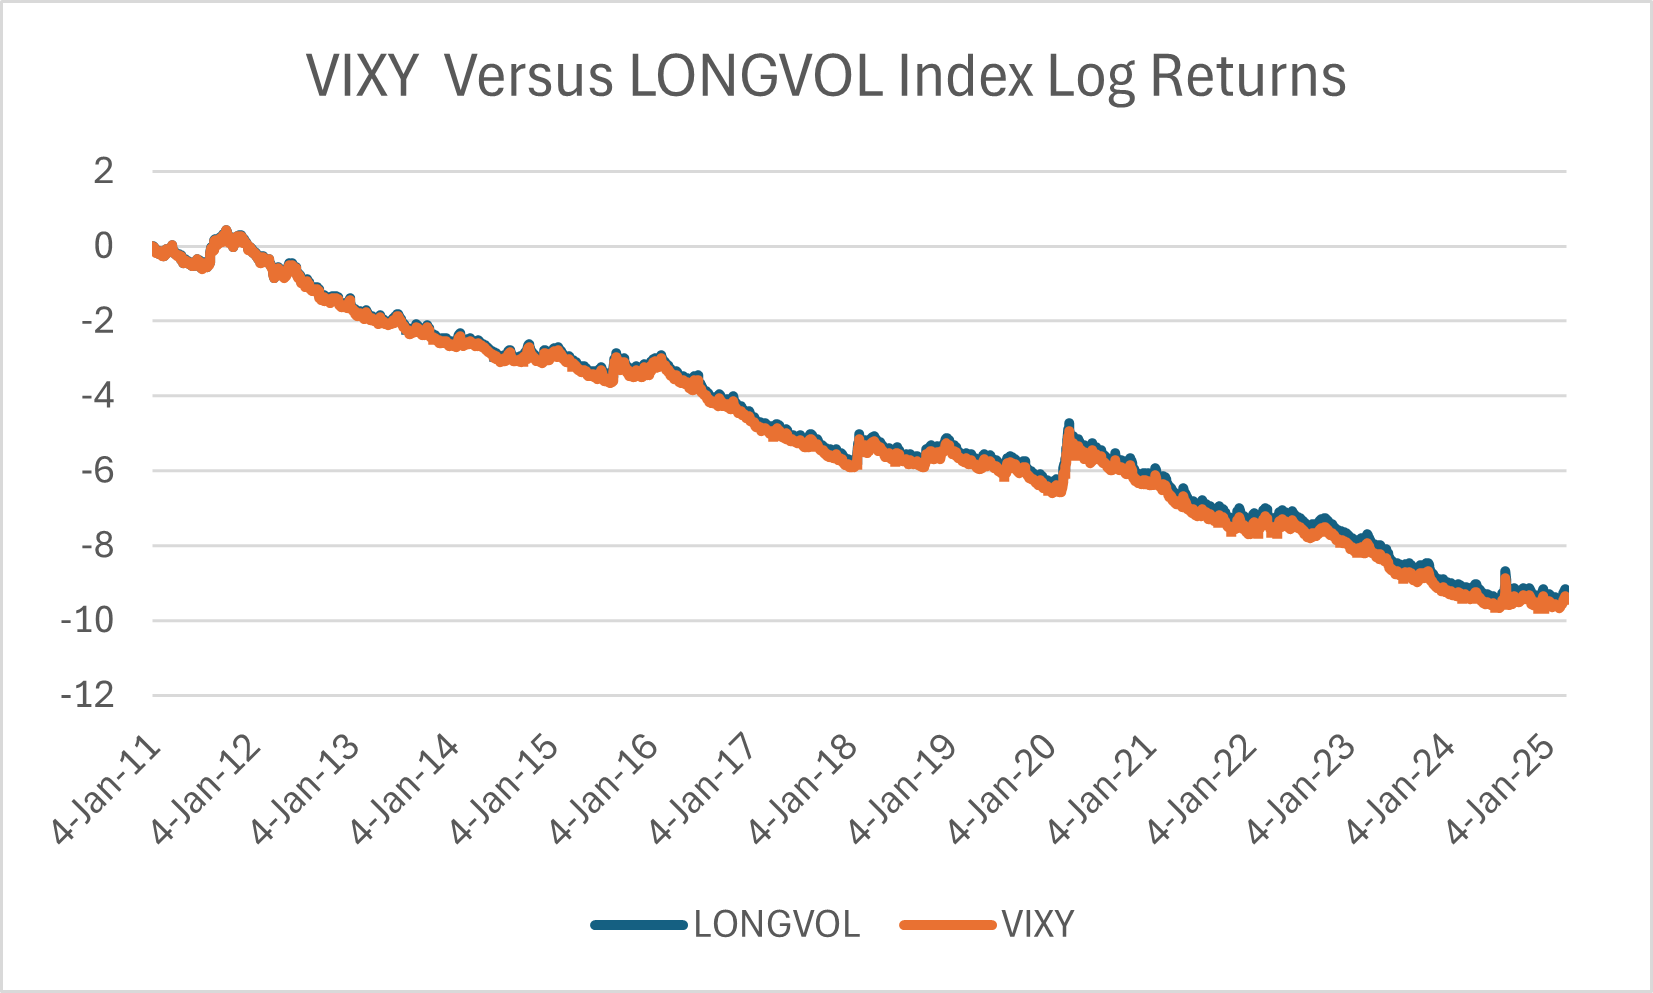
\includegraphics[width=\textwidth]{VIXYVersusLONGVOL.png}
\caption{VIXY Versus LONGVOL Index} \label{Fig-VIXYVersusLONGVOL}
\end{figure}
\noindent
The next graph shows the difference of log returns versus VIXY and LONGVOL.\\
\\
\begin{figure}[H]
\centering
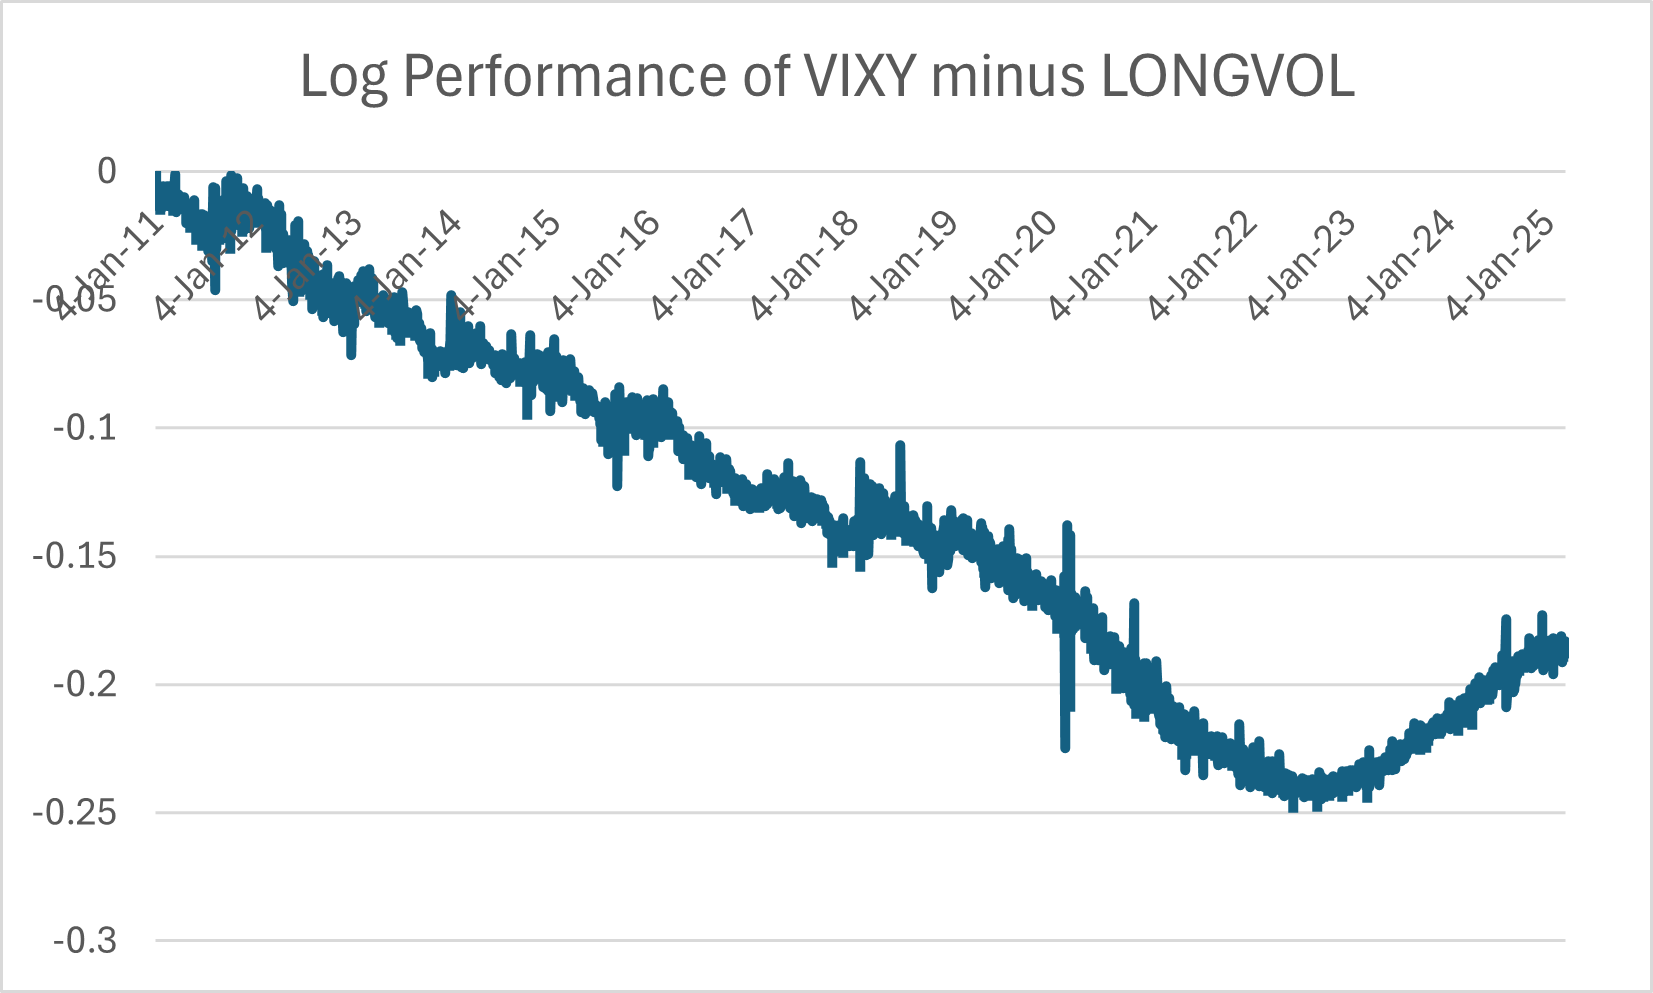
\includegraphics[width=\textwidth]{VIXYMinusLONGVOL.png}
\caption{VIXY Minus LONGVOL} \label{Fig-VIXYMinusLONGVOL}
\end{figure}
\noindent
\subsubsection{Expense Ratios} \label{ETFs-Benefits-Costs-ER}
Due to the frequent rebalancing, the management fee of volatility ETFs tends to be relatively high at around 0.95\% at the time of writing.

\subsubsection{Transaction Costs} \label{ETFs-Drawbacks-Costs-Transaction}
Due to the frequent rebalancing, the funds pay a lot of transaction fees and other costs similar to crossing the bid-ask spread. The following graph shows the difference of log performance between VIXY and LONGVOL with the expense ratio removed.\\
\\
\begin{figure}[H]
\centering
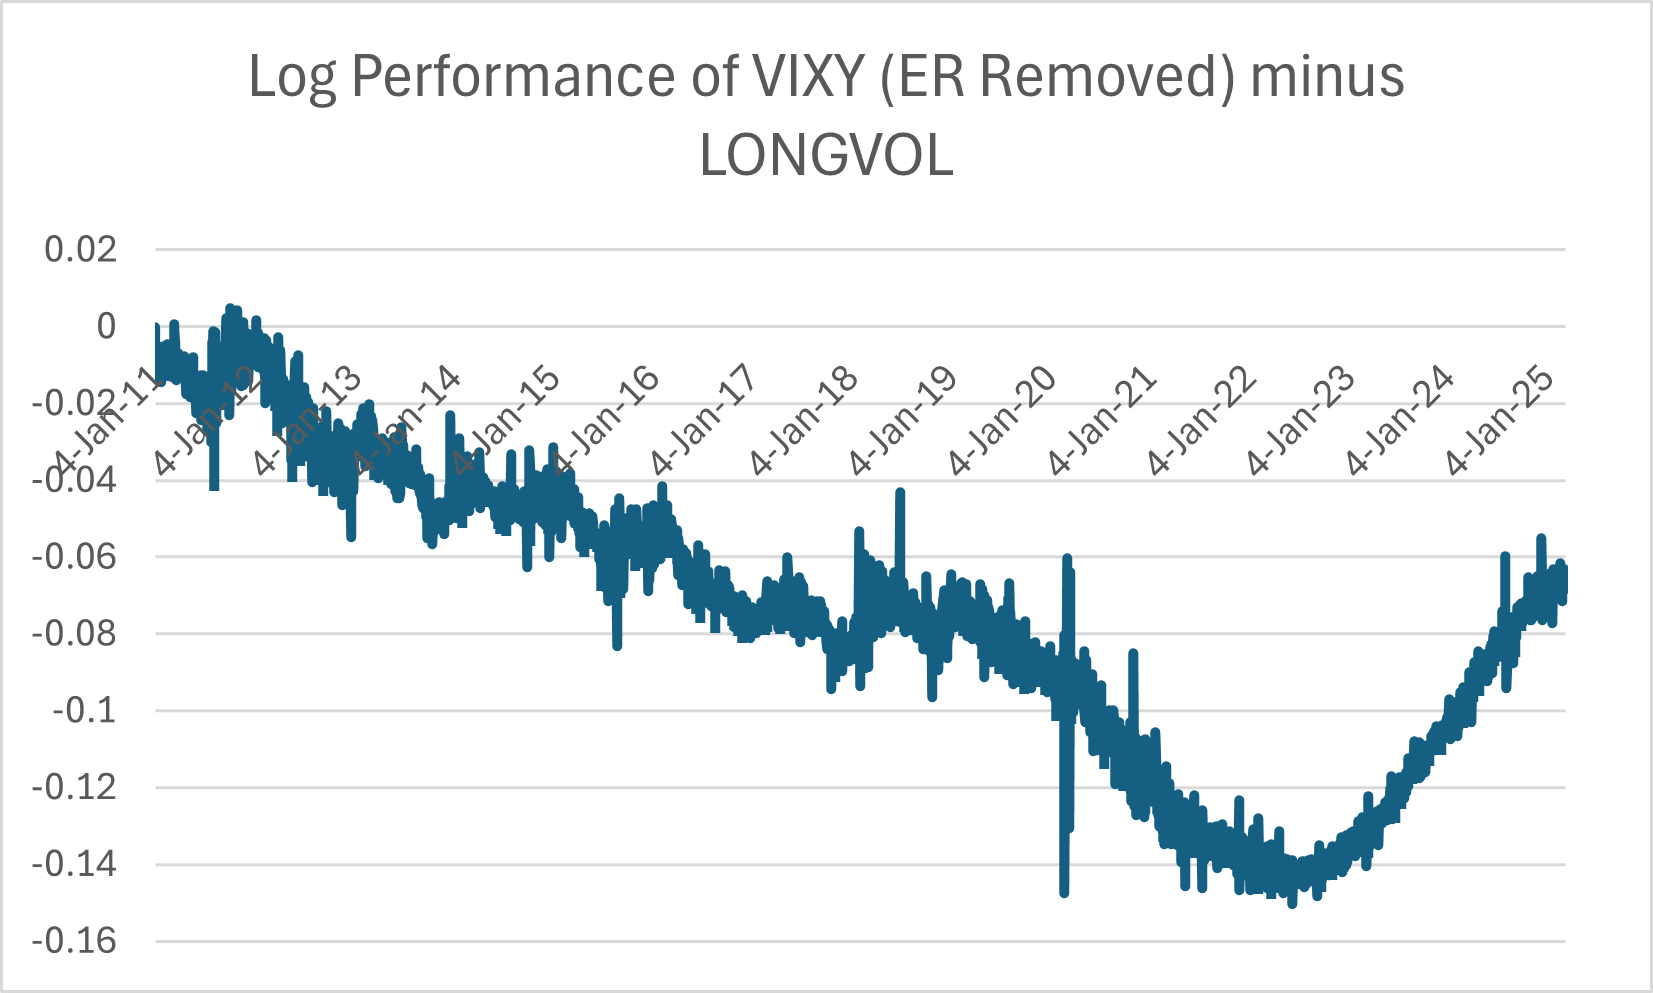
\includegraphics[width=\textwidth]{VIXYERRemovedMinusLONGVOL.png}
\caption{VIXY ER Removed Minus LONGVOL} \label{Fig-VIXYERRemVersusLONGVOL}
\end{figure}
\noindent

\subsection{Low Leverage Available on Short Volatility Funds} \label{ETFs-Drawbacks-Leverage}
Since shorting volatility futures is very risky, the short volatility funds have lower multipliers when compared to the long volatility ETFs. The multipliers of some volatility ETFs were reduced after the "Volmageddon" of 2018. Some short volatility ETFs have begun to purchase OTM VIX calls to reduce this risk (creating synthetic VIX puts as described in section \ref{Options}).\\
\\
The low multipliers reduce the amount of risk that can be taken using the ETFs. It is difficult to increase a portfolio's returns much higher the returns of the S\&P 500 using volatility ETFs.

\chapter{Investing In Volatility} \label{Investing}
The previous sections have explained the different tradable products involving the VIX. This section will describe multiple approaches to investing in volatility. It will explain the benefits and drawbacks to each approach, and it will provide some backtests and historical data to support each approach. Throughout the previous chapters, a consistent theme has been that short volatility is profitable over the long-term. Each of the approaches in this section are different ways to obtain short exposure to volatility.\\
\\
Some of the strategies described herein require active management. This does not imply that the strategies are speculative or meant for short-term trading. The intent of these strategies is to exploit the benefits of being short volatility over a long period. In other words, despite the active management of the strategies described in this section, these strategies are meant for investors investing over a long time period.

\section{Purchasing Short Volatility ETFs} \label{Investing-PurchETF}
\subsection{Benefits} \label{Investing-PurchETF-Benefit}
Purchasing short volatility ETFs is one of the easiest ways to get exposure to short volatility. If an investor is looking for an easy, buy-and-hold method of obtaining short volatility exposure, ETFs are one of the only options. 

\subsection{Drawbacks} \label{Investing-PurchETF-Drawback}
There are a few drawbacks. These ETFs:
\begin{itemize}
    \item Have a high expense ratio
    \item Pay a lot of transaction fees
    \item May provide a lower-than-required exposure to short volatility
    \item May not provide perfect exposure to the target index
\end{itemize}
The issues above are described further in section \ref{ETFs}.

\subsection{Historical Performance} \label{Investing-PurchETF-Historical}
The following chart shows the performance of SVXY from 2011 to 2025.\\
\\
\begin{figure}[H]
\centering
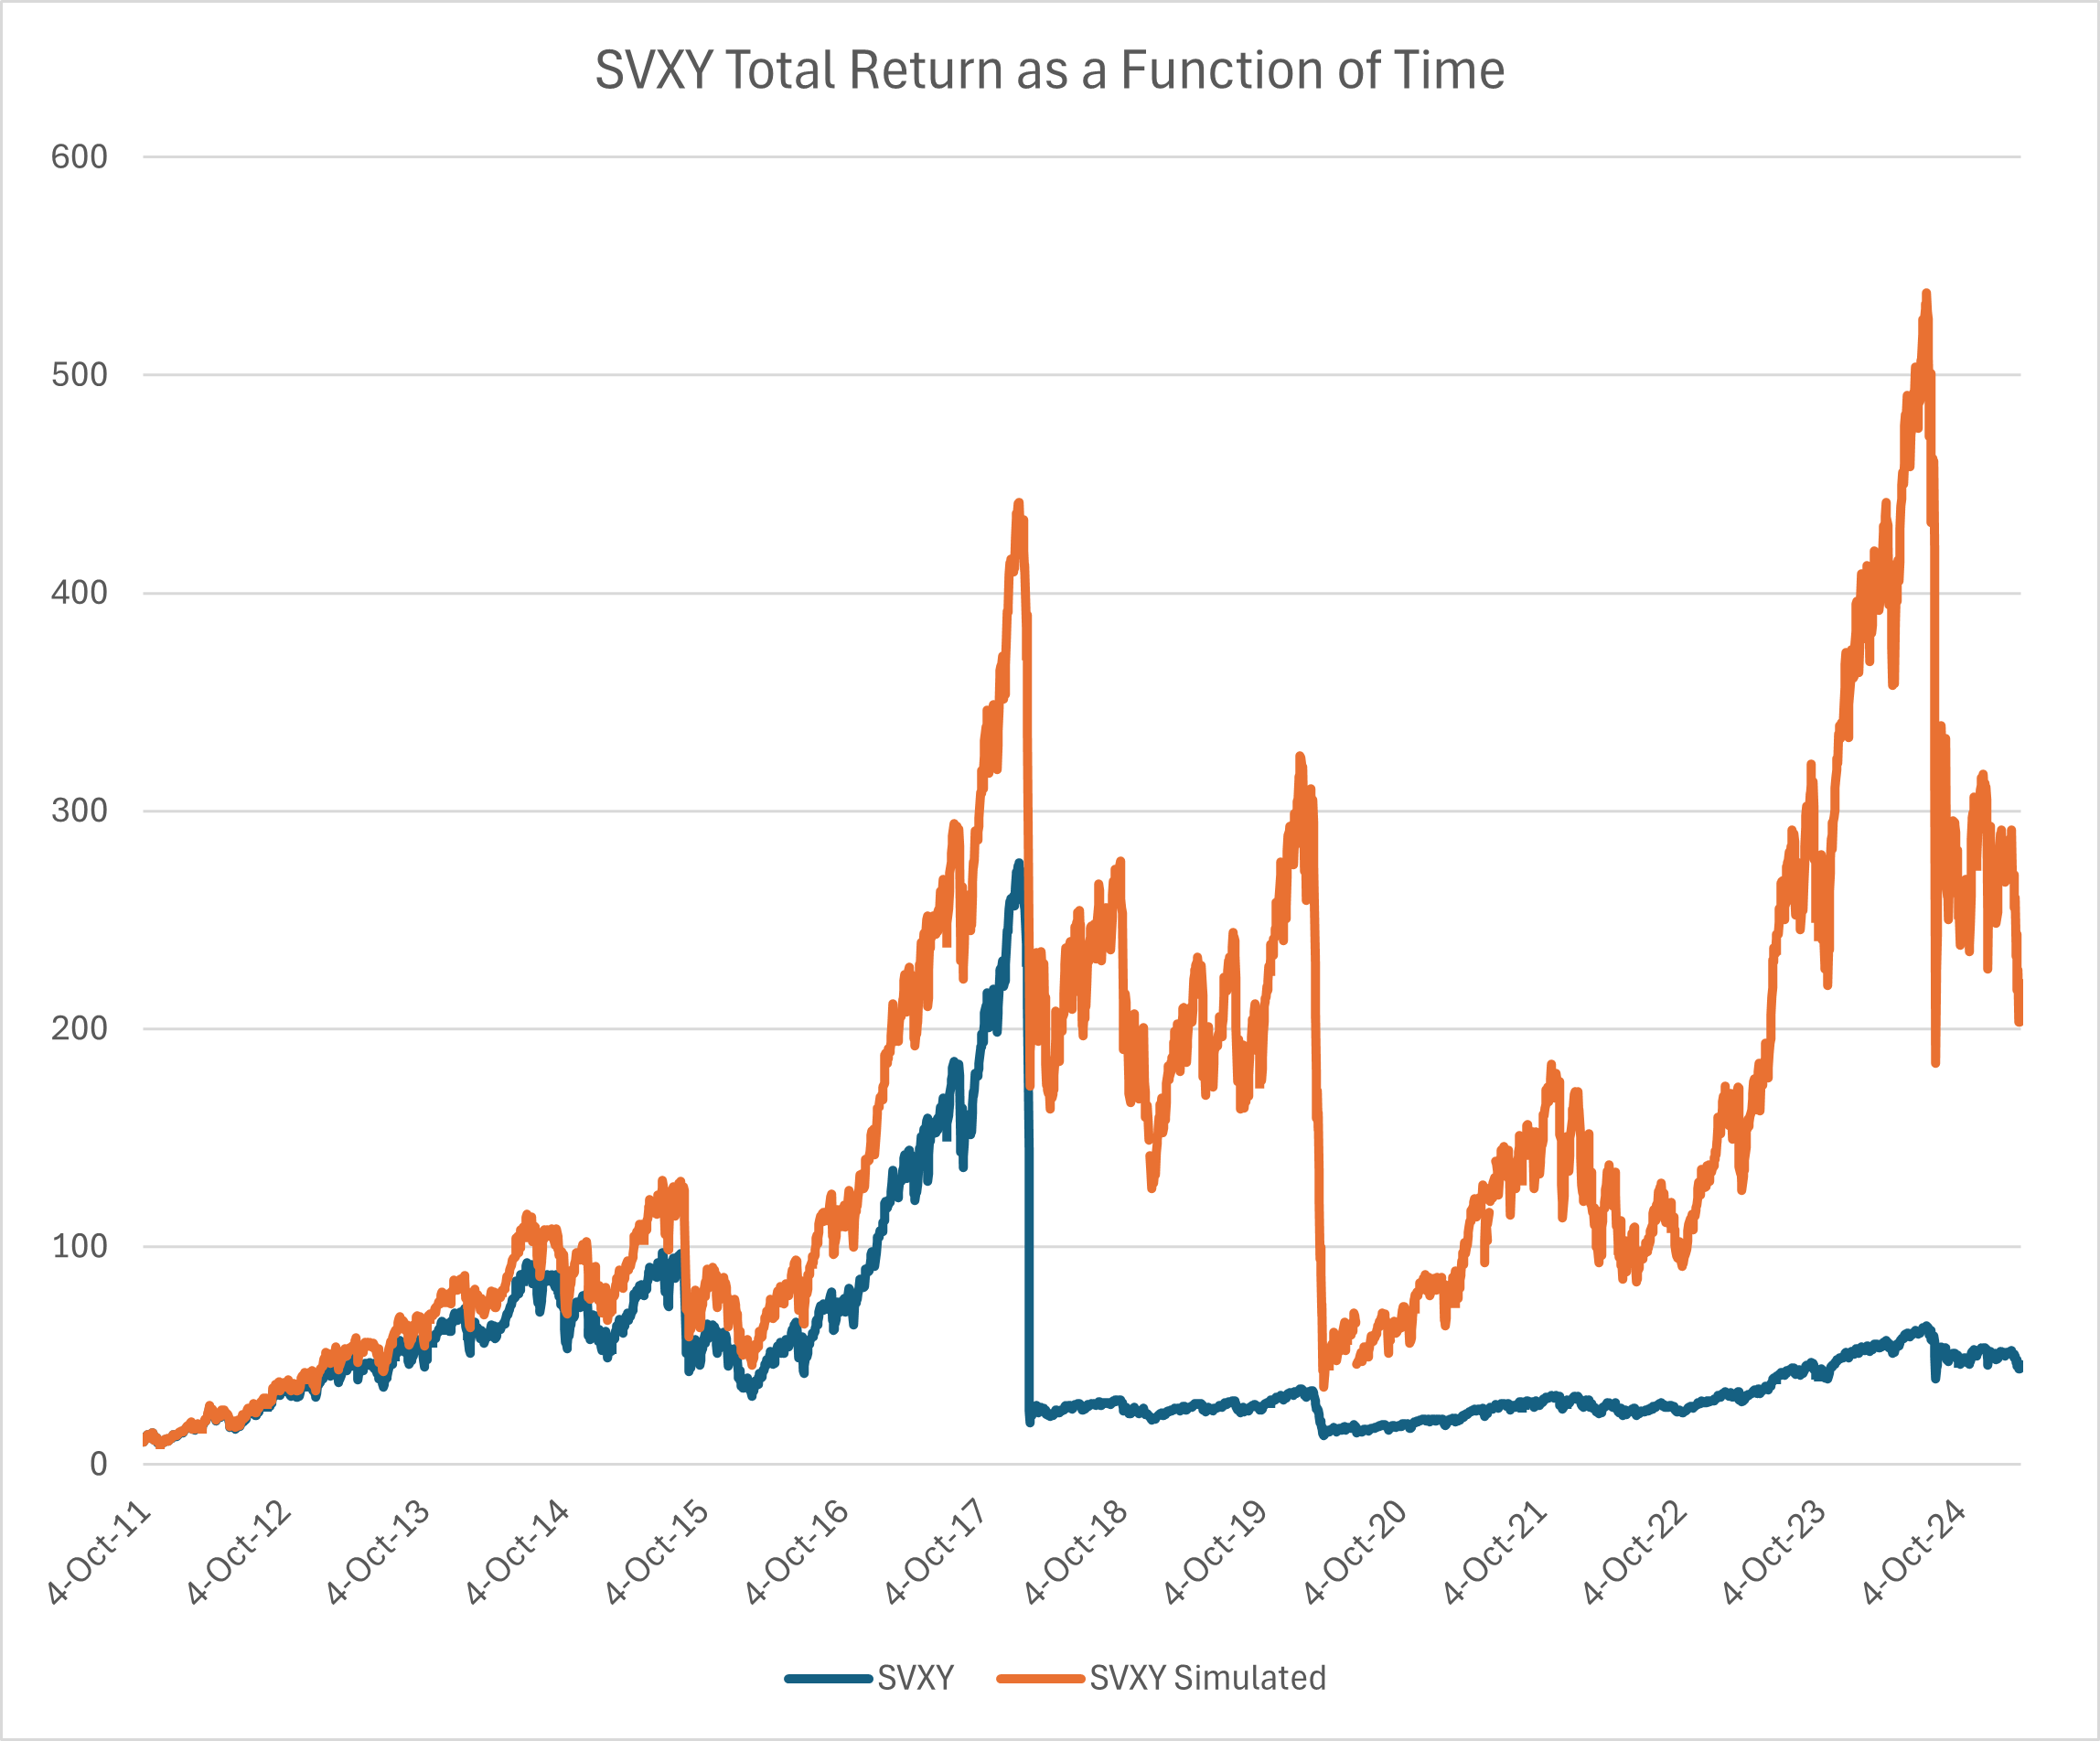
\includegraphics[width=\textwidth]{SVXY.png}
\caption{SVXY Versus SVXY Simulated} \label{Fig-SVXYVersusSIMSVXY}
\end{figure}
\noindent
This chart includes the Volmageddon event that occurred in 2018. Note that the multiplier of SVXY also changed in 2018 from -1x to -0.5x in response to Volmageddon. The SVXY Simulated line on the chart simulates SVXY as if the multiplier remained -1x. The provider of the SHORTVOL index data used to simulate SVXY also performed some adjustments during Volmaggedon to reduce its effect. The simulated SVXY takes into account the expense ratio of SVXY but does not account for the transaction costs the fund incurs when it trades.\\
\\
The following chart is the simulated returns of SVXY with a -0.5x multiplier from 2005 to 2025. The simulation crudely attempted to include the transaction costs incurred by the ETF the methodology is described in the appendix in Appendix B.\\
\\
\begin{figure}[H]
\centering
\includegraphics[width=\textwidth]{SimulatedSVXY.png}
\caption{Simulated SVXY} \label{Fig-SimSVXY}
\end{figure}
\noindent
Notably, the simulated fund only returned roughly 6.2\% per year over this period. To obtain higher returns, one would need to invest in an ETF with a higher multiplier. At the time of writing, the only short volatility ETF with a higher multiplier is SVIX. SVIX has a multiplier of -1x, but SVIX purchases calls to reduce the risk of tail events. The purchasing of calls eats into the expected returns of the ETF and therefore reduces the effective leverage of the ETF.\\
\\
The low expected returns does not make short volatility ETFs useless. Short volatility ETFs may be useful to investors with lower risk appetites or investors who wish to diversify across different asset classes. These ideas will be expounded further in section \ref{Conclusion-Benefits-Diversify}.

\section{Short Front-Month VIX Futures} \label{Investing-ShortFrontFut}
Another method of shorting volatility is shorting the front-month VIX futures and rolling each time the future expires. 

\subsection{Benefits} \label{Investing-ShortFrontFut-Benefit}
The benefits of this approach are listed below:
\begin{itemize}
    \item Since the portfolio is managed by the investor and not the fund, there are no management fees.
    \item This approach has a lower frequency of trading when compared to the ETFs. This reduces transaction costs.
    \item Futures do not require an initial capital outlay. This approach allows an investor to efficiently increase risk.
\end{itemize}

\subsection{Drawbacks} \label{Investing-ShortFrontFut-Drawback}
The drawbacks of this approach are listed below:
\begin{itemize}
    \item The sensitivity of the portfolio to volatility is non-constant. As the current future nears expiration, the portfolio becomes more sensitive to movements in the spot VIX. Non-constant sensitivity can make risk management difficult.
    \item This approach requires trading at least once a month. Active management is subject to additional behavioral risks than buy-and-hold investing.
    \item Exposure to the VIX increases as the VIX increases and exposure to the VIX decreases as the VIX decreases. This poses a challenge from a risk management perspective.
\end{itemize}
\newpage
\subsection{Historical Performance} \label{Investing-ShortFrontFut-Historical}
The following chart is a simulated portfolio consisting of two positions: a 100\% allocation to short-term bonds and a position in short front-month VIX futures such that the notional value of the futures contracts is 20\% of the portfolio's value.\\
\\
\begin{figure}[H]
\centering
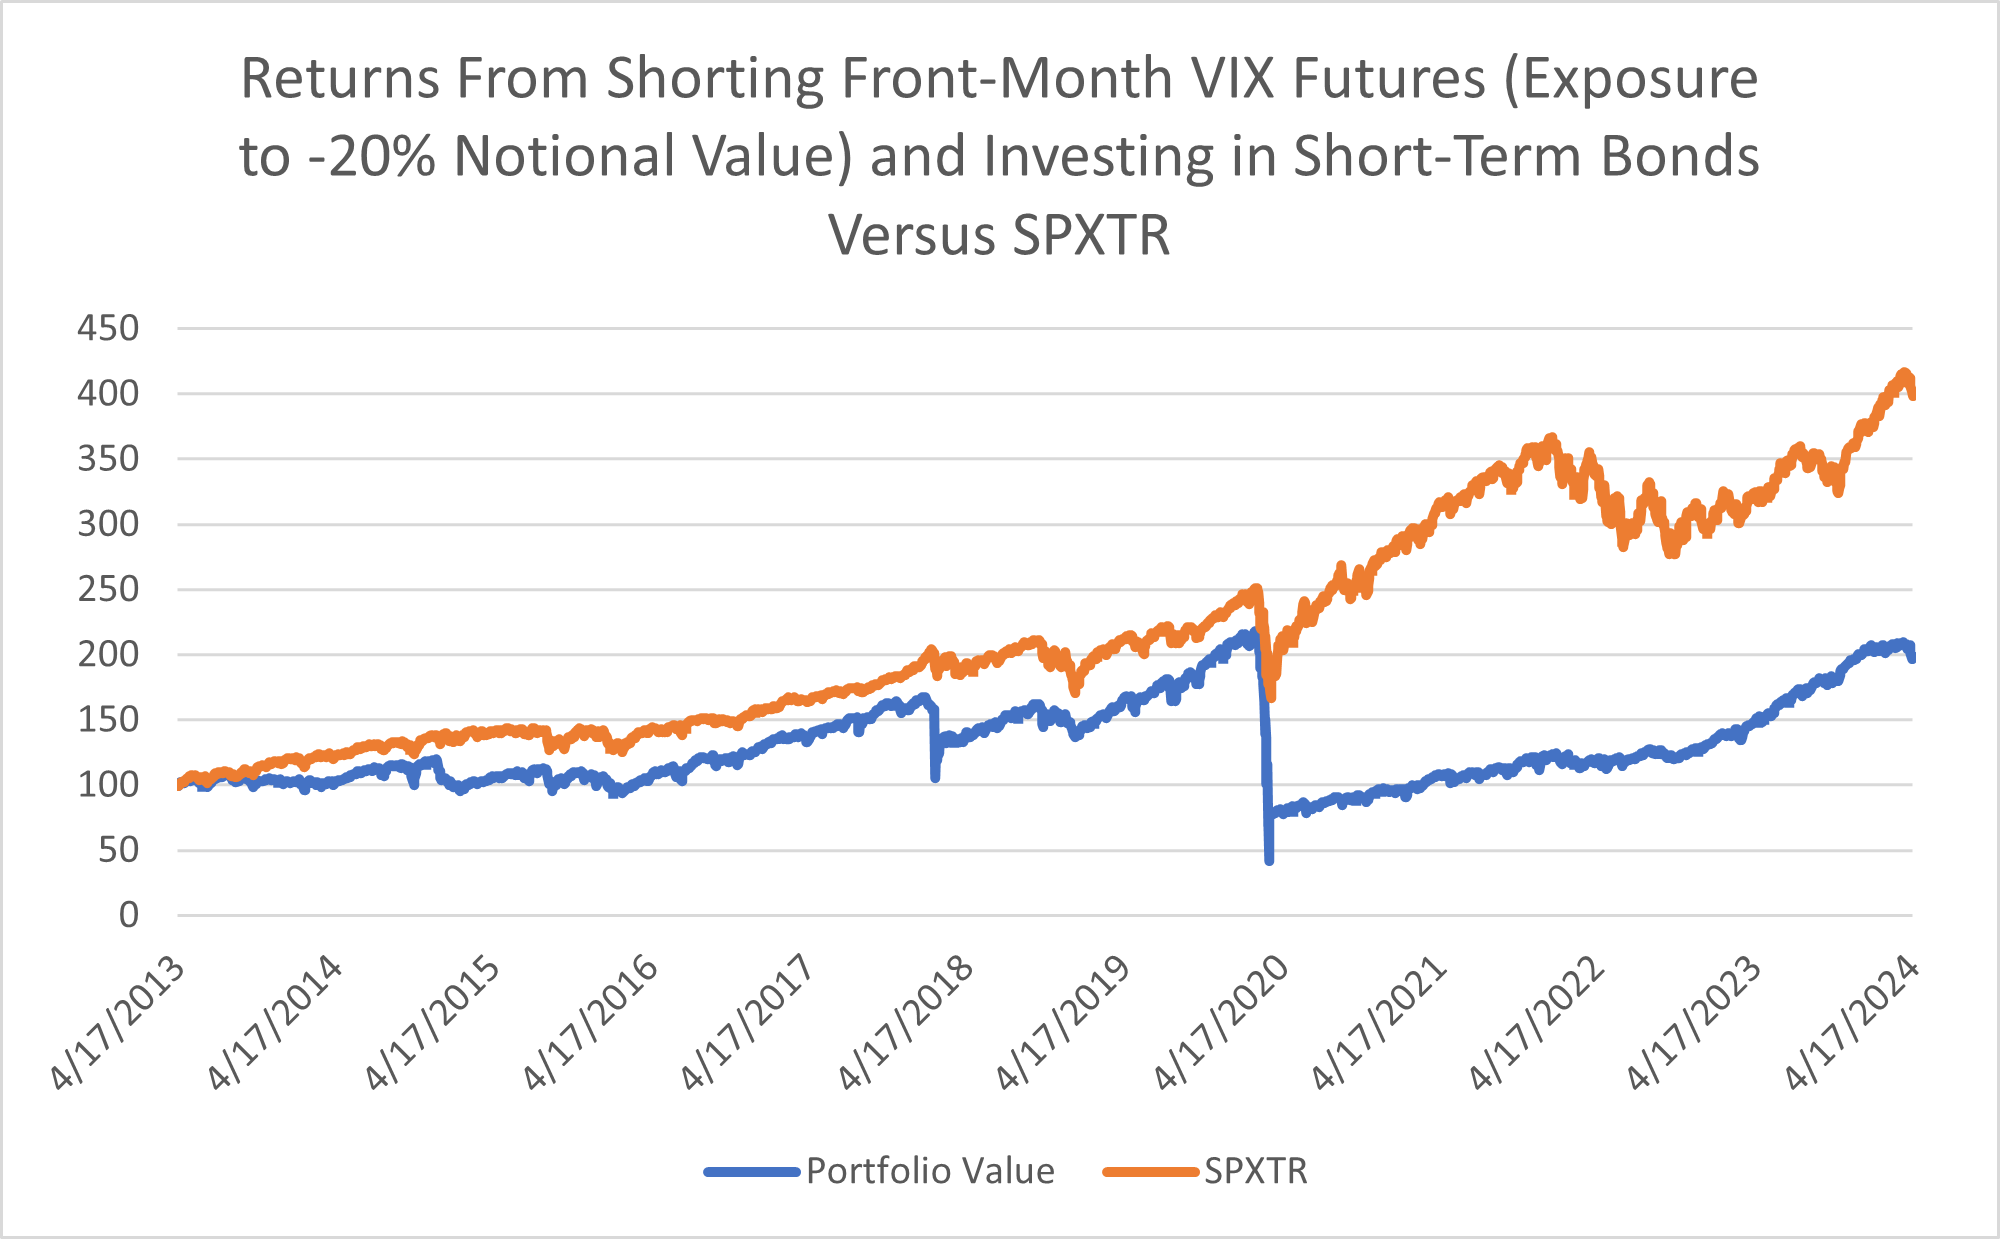
\includegraphics[width=\textwidth]{ShortingFrontMonthFutures.png}
\caption{Shorting Front-Month VIX Futures} \label{Fig-ShortFrontMonth}
\end{figure}
\noindent
The performance of the simulated portfolio is very similar to the returns from holding the S\&P 500 up until the crash in 2020. The effect of the crash on the portfolio is a perfect example of the increased sensitivity of a futures position to the spot VIX as the expiration nears. The steep decrease in the value of the portfolio was caused by the VIX increasing from roughly 20 to 80 as the VIX futures approached expiration. A view of the portfolio value, the VIX, the time to expiration of the front-month contracts, and the front-month VIX futures are shown in the graph below:\\
\\
\begin{figure}[H]
\centering
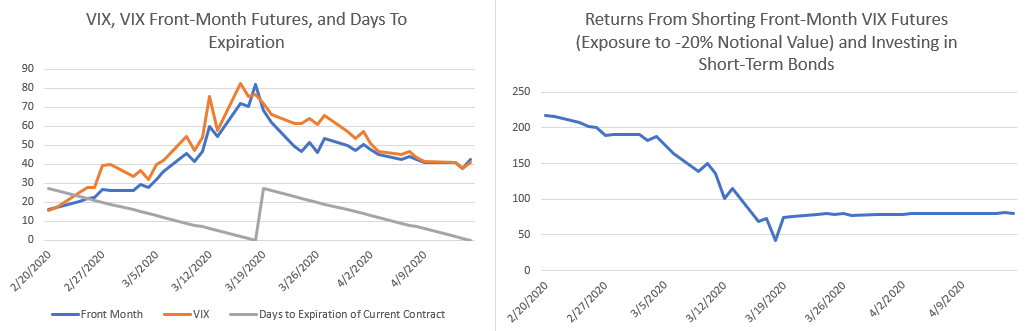
\includegraphics[width=\textwidth]{ShortingVolatilityDuringCovid.png}
\caption{Shorting Volatility During COVID} \label{Fig-ShortVolDuringCOVID}
\end{figure}
\noindent
The probability of the timing of a crash occurring at the same time as the expiration of the futures is extraordinarily low, but, as shown above, non-zero. The next approach to shorting volatility will reduce the effect of these Black Swan events at the cost of expected returns.

\subsection{Additional Note} \label{Investing-ShortFrontFut-Note}
There are many parameters to adjust when implementing this strategy. An investor can choose to roll across different months or short with a different notional exposure than 20\%. 

\section{VIX Puts} \label{Investing-VIXPut}
As mentioned in section \ref{Options}, a put is synthetically equivalent to shorting the underlying, purchasing bonds, and purchasing a call at the same strike as the put that the trader is synthetically replicating. Section \ref{Options} mentioned that the extrinsic value of an option can be viewed as a cost of the option's exposure. This claim is slightly inaccurate and will be addressed with more nuance in this section.\\
\\
Much like the pricing of VIX futures, the extrinsic value of options can be viewed in two parts: the fair value of the extrinsic value and the risk premium. The fair value represents the fair value of the asymmetric payoff of the option assuming reasonable expectations of the underlying and its probability distribution. The risk premium represents the payment to the participant taking the risk by selling the option. This primer will not attempt to differentiate between the fair value and the risk premium. Using the intuition behind the expected returns from shorting VIX futures, current VIX put prices, and current future prices, it is easy to calculate which VIX options have positive expected returns even with the assumption that 100\% of an option's extrinsic value is risk premium.\\
\\
The goal of purchasing VIX puts is to obtain short exposure to volatility while maintaining positive expected returns. There are several parameters that can be adjusted with this strategy: allocation, strike price, and time to expiration. Decreasing the strike price increases the leverage and the exposure to short volatility but decreases the expected risk-adjusted returns. To reduce the risk of subjectivity (behavioural risk) impacting investing decisions, it's best to select the strike price based on objective and measurable criteria.

\subsection{Benefits} \label{Investing-VIXPut-Benefit}
\begin{itemize}
    \item This strategy has defined risk.
    \item This strategy allows an investor to efficiently add risk to their portfolio even in restricted accounts such as retirement accounts.
\end{itemize}

\subsection{Drawbacks} \label{Investing-VIXPut-Drawbacks}
\begin{itemize}
    \item As the VIX increases the exposure to the position decreases.
    \item The sensitivity of the portfolio to volatility is non-constant. As the current future nears expiration, the portfolio becomes more sensitive to movements in the spot VIX. The non-constant sensitivity can make risk management difficult.
    \item This approach requires trading at least once a month. Active management is subject to additional behavioral risks than buy-and-hold investing.
\end{itemize}

\subsection{Historical Data} \label{Investing-VIXPut-Historical}
 The following backtest allocated 20\% of their portfolio to a monthly VIX option whose strike was closest to 1.9x the current VIX futures price. Each time the current VIX option expired, a new one was purchased meeting the same criteria (similar the the front-month VIX future strategy discussed in section \ref{Investing-ShortFrontFut}).\\
\\
\begin{figure}[H]
\centering
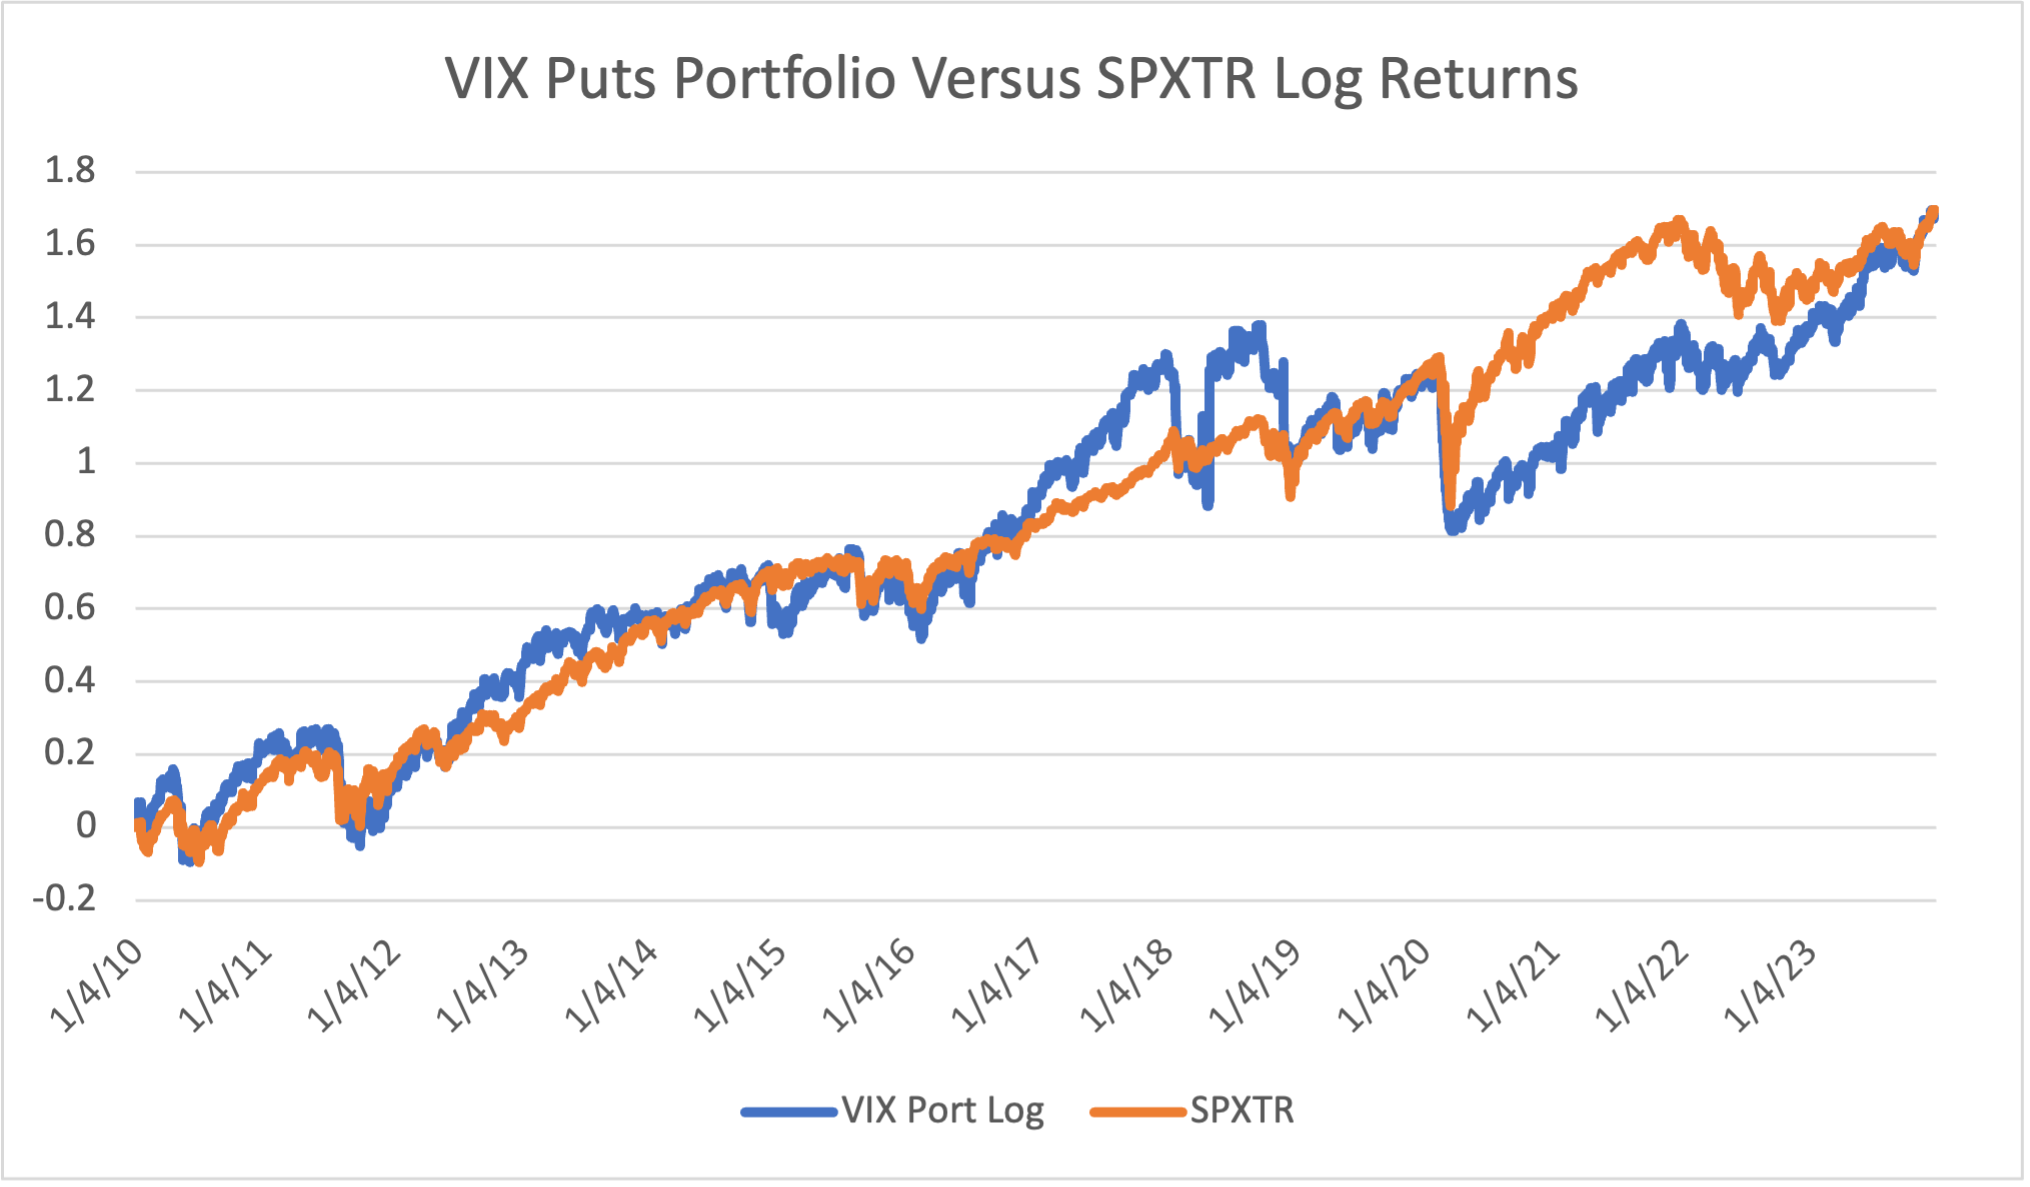
\includegraphics[width=\textwidth]{VIXPuts.png}
\caption{VIX Puts Versus SPXTR} \label{Fig-VIXPutsVsSPXTR}
\end{figure}
\noindent
Note: The rest of the 80\% of the portfolio was left uninvested. This means that an investor can obtain returns similar to the S\&P 500 with only a 20\% allocation in their portfolio. Further adjustment of the parameters would allow an investor to increase or decrease their exposure to their risk tolerance as well as pair the strategy with other investments. This idea is mentioned briefly in section \ref{Conclusion-Benefits-Diversify}.\\
\\
The parameters of this backtest were chosen to match the returns of the S\&P 500 to make it easier to visually compare the volatility of the two strategies. Visually, the volatility of the two strategies appear to be roughly the same. Therefore, the risk-adjusted returns are similar based on this backtest.


\section{Synthetic VIX Puts} \label{Investing-SyntheticPut}
As mentioned in section \ref{Investing-VIXPut}, a VIX put is synthetically equal to shorting a VIX future, bonds, and purchasing a call (Note: At the time of writing, the contract multipliers between a VIX future and a VIX put are different by a factor of 10). Creating synthetic puts by shorting VIX futures and purchasing calls reduces the initial capital outlay. This allows an investor to invest the extra cash in different opportunities. This strategy is very similar to the VIX puts, for this reason, the benefits and drawbacks will focus on the difference between synthetic VIX puts and real VIX puts. There will not be a historical data section.

\subsection{Benefits Compared to VIX Puts} \label{Investing-SyntheticPut-Benefit}
\begin{itemize}
    \item Lower initial capital outlay. An investor can invest cash in other opportunities.
    \item OTM calls are generally more liquid than ITM puts (however, the net transaction cost might be higher anyways. See the drawbacks section.)
\end{itemize}

\subsection{Drawbacks Compared to VIX Puts} \label{Investing-SyntheticPut-Drawbacks}
\begin{itemize}
    \item Higher fees. The investor needs to pay the transaction fee of both the short future and the long calls.
    \item Higher transaction cost due to bid-ask spread. The investor must short the VIX future and purchase the long calls. The minimum tick of VIX futures is non-negligible.
    \item The investor must have a futures trading account.
\end{itemize}

\section{Short VIX Calls} \label{Investing-ShortVIXCalls}
Short VIX calls have the benefit of being both short volatility and short volatility of volatility. Similar to the VIX puts, there are many parameters that can be adjusted: notional exposure, strike price, and time to expiration. The selection of these parameters affect the expected returns and exposure to tail risk. A low strike price will behave similarly to a short VIX future. A high strike will have consistent returns except in the event of a significant spike in volatility.\\
\\
The returns and volatility of a short VIX call strategy strongly depend on the allocation and the strike selection. For this reason, a backtest will not be included in this primer.

\section{Shorting Long Volatility ETFs} \label{Investing-ShortETF}
At the time of writing, the cost to borrow of long volatility ETFs is too high to make shorting long volatility ETFs worthwhile. It is more efficient to purchase short volatility ETFs than to short long volatility ETFs. For this reason, this topic will not be explored further in this primer.\\
\\
Note: This does not mean that the expected returns of shorting long volatility ETFs is negative. However, the methods described in this section above are much more efficient than shorting long volatility ETFs.

\section{Purchasing Puts on Long Volatility ETFs} \label{Investing-PutsETF}
The cost to borrow of the underlying is generally priced into the price of puts. For this reason, purchasing puts on long volatility ETFs is less efficient than the methods previously described in this section. For this reason, this topic will not be explored further in this primer.

\section{Shorting SPX Options} \label{Investing-ShortSPXOpts}
Section \ref{Options-BSM} explained that the purchasing of options generally has exposure to the implied volatility of the options and, in most cases, realized volatility of the underlying.\\
\\
Throughout this primer, options have been used to obtain short exposure to volatility or volatility derivatives. Using option's terminology: the goal has been to purchase or sell options that created a net negative delta on a volatility index or ETF. The goal of shorting SPX options is different; it's to have near-zero delta and negative vega.\\
\\
There are many methods of using options to get exposure to short vega. A few examples are: iron condors, short straddles/strangles (with or without delta hedging/gamma scalping), or short puts/short calls with delta hedging/gamma scalping. The maintenance of these options strategies is a complicated subject and is not in the scope of this primer.

\chapter{Conclusion} \label{Conclusion}
In conclusion, short-volatility strategies can provide a long-term investor with certain desirable characteristics. This primer aimed to expose the reader to the idea of adding short volatility exposure to a portfolio without explicitly endorsing it or describing specific implementation details. \\
\\
This section will review some of the benefits and drawbacks to adding short volatility to a portfolio. This section should not be interpreted as a recommendation to include short volatility exposure. \\
\\
Risk management is a very important part of shorting volatility. Managing the risk of short volatility positions is very complicated and was only discussed at a surface level in this primer. It is important to note that while historical data is presented often in this primer, historical data may not accurately represent future results and cannot be relied on as a basis for risk management practices. \\
\\
If, after reading this section, a reader is inclined to add short volatility exposure to their portfolio, it would be best to research risk management principles or make short volatility a very small portion of their portfolio.

\section{Benefits} \label{Conclusion-Benefits}
\subsection{Increasing a Portfolio's Risk and Expected Returns} \label{Conclusion-Benefits-IncreaseEV}
Section \ref{Futures-VIXFuts-Selling} briefly explains why the risk-adjusted returns of shorting volatility must be similar to the risk-adjusted returns of investing in the asset that the volatility is based off of (in the case of VIX, the S\&P 500). The volatility of the VIX (and therefore the risk) is much higher than the S\&P 500. Therefore, the expected returns from shorting the VIX must be higher than the returns of the S\&P 500.\\
\\
An investor could use the strategies described herein to increase the expected returns of their portfolio in a very efficient manner. 

\subsection{Diversification} \label{Conclusion-Benefits-Diversify}
While the VIX is ultimately a derivative of the S\&P 500, the VIX is not 100\% correlated with the S\&P 500. For this reason, a carefully constructed portfolio of short volatility exposure and the S\&P 500 may reduce the overall variance of the portfolio while maintaining the expected returns (this increases the risk-adjusted returns). This fact is based on the following inequality using two random variables $X$ and $Y$:
\begin{equation}
Var(X+Y) \leq \frac{1}{2}(Var(X) + Var(Y))
\end{equation} \label{Eq-VarianceSum}
It is important to note that short-volatility portfolios tend to have lower beta during normal market conditions and very high beta during market crashes. In other words, a short-volatility portfolio tends to have lower-than-market volatility in normal market conditions, and significantly higher-than-market volatility during a market crash. As shown in the historical data subsections in section \ref{Investing}, short volatility strategies tend to be stable for long periods, but they tend to have infrequent and significant drawdowns.  \\
\\
It is important to view portfolios containing short volatility positions from a risk perspective rather than an allocation perspective. For example, a 10\% allocation to short volatility - depending on the method selected - may represent a significant of a portfolio's risk. Unfortunately, quantifying the relative risk of a short volatility position to a portfolio is difficult and will not be discussed in this primer.

\section{Drawbacks} \label{Conclusion-Drawback}
\subsection{High Correlation During Crashes} \label{Conclusion-Drawback-Correlation}
Short volatility strategies provide some diversification to the market when the market is calm. However, during a market crash, both the market and short volatility portfolios will fall sharply. As mentioned, this fact makes managing risk difficult. 

\subsection{Tail Risk} \label{Conclusion-Drawback-TailRisk}
The idea that the VIX is highly risky and volatile is a constant theme throughout this primer. "Selling insurance" by shorting volatility exposes the seller to significant risk because the VIX spikes significantly during tail events. The reason shorting volatility has positive expected returns is due to this risk. Therefore, attempts to hedge the tail risk will significantly reduce the expected returns of shorting volatility. 

\subsection{Active Management} \label{Conclusion-Drawback-Management}
Many of the strategies described in this primer require active management and maintenance. Active management may increase market-related anxiety and may introduce behavior risk. Actively managed portfolios also consume the time of the investor.

\subsection{Taxes} \label{Conclusion-Drawback-Taxes}
In the US, the taxation of short-volatility strategies may be worse than long-term buy-and-hold strategies. VIX futures and options are Section 1256 contracts. At the end of each tax year, gains and losses on VIX contracts are "realized" (marked to market) at 40\% STCG and 60\% LTCG regardless of the holding period and regardless of whether the gain was realized.\\
\\
This forced realization of gains (and taxation) reduces the compounding of the gains from short volatility. For this reason, it may be advantageous to add short volatility exposure to a tax-advantaged account rather than a taxable account.






\chapter{Appendix A} \label{AppendixA}
\section{Quantifying Risk Premium - Smoothing} \label{AppendixA-Smooting}
To create the chart in section \ref{Futures-Quantify}, data containing dates, futures prices, and their expiration dates was collected. From this data, a set of days to expiration and futures price from all of the futures was derived. \\
\\
Due to the contract schedule of VIX futures, there were discontinuities in the data. To smooth the discontinuities, the data was convolved with $\{\frac{1}{5}(u(t-2.5)-u(t+2.5))$ where $u(t)$ is the unit step function. Once smoothed, the resulting data was graphed as a function of days to expiration. 
\backmatter
\end{document}
